\chapter{Multilevel Bayesian joint model of longitudinal and binary outcomes}\label{chp2}

In this chapter, we illustrate our proposed multilevel Bayesian joint model (JM) that encompasses the Linear Mixed Effect (LME) model with a Gaussian process and the GLMM with a flexible link function. This chapter is organized as follows. In Section \ref{sec:chp2_mov}, we emphasize the motivation. In Section \ref{sec:chp2_mod}, we introduce the methodology, including model framework, Bayesian inference, predictive metrics and model comparison criterion. In Section \ref{sec:chp2_sim} and \ref{sec:chp2_app}, we illustrate simulation studies and application results, respectively. Lastly, we conclude our study with remarks and discussions in Section \ref{sec:chp2_con}. 

\section{Motivation} \label{sec:chp2_mov}

Although joint modeling has been a useful strategy in modern longitudinal analysis, applications to hierarchical longitudinal studies have been less frequent, particularly with respect to a binary process, which is commonly specified by a Generalized Linear Mixed Model (GLMM). Moreover, an added complexity occurs when the Gaussian process for irregular visits and flexible link function are involved to facilitate estimation and prediction. To the best of our knowledge, these two key challenges have not been considered together in the existing joint modeling approaches. 

For this cause, we propose a joint model that unites a LME submodel for the evolution of ppFEV1 and a GLMM for the occurrence of PE in individuals who have already experienced a PE event prior to follow up during our analysis time frame. Both center- and individual-level random intercepts are the basis of latent associations between these two submodels. In addition, we employ a stationary exponential correlation function for ppFEV1 to allow for longstanding correlation and intrinsic nonlinearity (\cite{Szczesniak2017}) and apply flexible link functions (\cite{Jiang2013}) for PE occurrence, which comprise both symmetric and asymmetric link functions to capture the underlying skewness of responses. To summarize, our motivation is threefold: i) compare common links with the flexible link; ii) quantify biases caused by ignoring center effect in a multicenter cohort analysis; iii) evaluate prognostic utility of the proposed novel joint model. 


\section{Model Framework} \label{sec:chp2_mod}

\subsection{The Joint Model}

Our proposed multilevel shared random effects joint model is expressed as 
\begin{equation} \label{eq:chp2_jm}
    \begin{gathered}
    Y_{lij}=\bm{X}_{li}(t_{lij})\bm{\alpha}+b_l+U_{li}+W_{li}(t_{lij}) + \epsilon_{lij}, \\
    Pr(R_{lij}=1)=F_{sp}\big(\bm{V}_{li}(t_{lij})\bm{\beta}+\rho_1 b_l + \rho_2 U_{li}; r_l\big)
    \end{gathered}
\end{equation}
where $Y_{lij}$ denotes continuous longitudinal profiles and $R_{lij}$ represents the binary response observed at time point $t_{lij}$ for subject $i$ from center $l$, with $l=1, \dots, L; i=1, \dots, n_l; j=1, \dots, n_{li}$. $\bm{X}_{li}(t_{lij})$ and $\bm{V}_{li}(t_{lij})$ denote row vectors of explanatory variables; $\bm{\alpha}$ and $\bm{\beta}$ are corresponding unknown coefficients. Between-center and between-patient heterogeneity are incorporated by random intercept terms $b_l$ and $U_{li}$, allowing for the assumption to be independent and identically distributed (i.i.d.) from $ N(0,\sigma_b^2)$ and $N(0,\sigma_u^2)$, respectively. A random-intercept model rather than the random intercept-and-slope model (\cite{Laird1982}) is adapted, because the latter is too rigid to capture the pattern of variability in ppFEV1 over longer periods of time \cite{TaylorRobinson2012}. The stochastic process $\bm{W}_{li}(t)$ describes how individual lung function varies over time and is assumed to be independent copies of a zero-mean, continuous-time stationary Gaussian process with the covariance function defined as 
\begin{equation}\label{eq:chp2_w}
Cov(W_{li}(t),W_{li}(s))=\tau^2 exp \big (-|t-s| \cdot \rho \big)
\end{equation}
where $t$ and $s$ are two arbitrary time points, $\rho$ represents the inverse of a range parameter and $\tau$ is the scale parameter for exponential correlation. A common concept for nugget factor $1-\mbox{nugget}=\frac{\tau^2}{\sigma^2 + \tau^2}$ incorporates both scale parameters $\tau$ and $\sigma$, with measurement error $\bm{\epsilon}$ following $N(0,\sigma^2)$. Furthermore, we assume that $\bm{b}$, $\bm{U}$ and $\bm{\epsilon}$ are mutually independent. 

Let $R_{lij}$ be a Bernoulli random variable with probability of PE occurrence $Pr(R_{lij}=1)$. $F_{sp}\big(g(\cdot); r_l\big)$ denotes a cumulative distribution function of a known symmetric power family with a linear function of covariates $g(\cdot)=\bm{V}_{li}(t_{lij})\bm{\beta}+\rho_1 b_l + \rho_2 U_{li}$ and center-specific power parameter $r_l$. Its inverse function $F^{-1}_{sp}$ is well known as a flexible symmetric power link function, which will be addressed in the next section. Parameters $\rho_1$ and $\rho_2$ measure the strength of the association through shared random components $b_l$ and $U_{li}$ between the two submodels.

\subsection{Symmetric Power Link Family}

\cite{Jiang2013} proposed a general class of power link functions, allowing flexible skewness in both positive and negative directions, while retaining the symmetric baseline link function as a special case. Let $F^{-1}_0$ be a symmetric baseline link function with corresponding cumulative distribution function (cdf) $F_0$, then symmetric power link family is defined as

\begin{equation} \label{eq:ch2_Fsp}
  F_{sp}(x;r)=F_0^r(\frac{x}{r})I_{(0,1]}(r)+\big[1-F^{1/r}_0(-rx)\big]I_{(1,+\infty)}(r),    
\end{equation}
where $I_A(r)$ is an indicator function with 1, when $r \in A$ and 0, otherwise. $x \in (-\infty, +\infty)$ denotes the linear function of predictors and $r$ is called by power parameter. The inverse transformation $x=F^{-1}_{sp}(\pi)$ is well known as the symmetric power link with $\pi \in [0,1]$. However, we are in favor of $F_{sp}$ because the probability of event occurrence $Pr(R_{lij}=1)=F_{sp}\big(g(\cdot);r_l\big)$. Particularly, $F_{sp}$ becomes cdf of splogit link when $F_0$ follows a Logistic distribution with location=0 and scale=1, and the cdf of spep link when $F_0$ follows a Laplace distribution location=0 and scale=1, as shown in Equation \ref{eq:F0}. 

\begin{align}
& F_0= \left \{\begin{array}{ll}
  F_{\mbox{logistic}}(x|\mu=0, s=1)= \frac{1}{1+exp(-x)}\\
  F_{\mbox{laplace}}(x|\mu=0, b=1)=\frac{exp(x)}{2}I_{(-\infty,0)}(x)+\big(1-\frac{exp(x)}{2}\big)I_{[0, +\infty)}(x)
\end{array}\right.
\label{eq:F0}
\end{align}

Figure \ref{fig:Chp2_cdf_sp} illustrates the skewness of response probability given covariate $x$ is symmetric about zero. Particularly, splogit reduces to the logit link when power parameter $r=1$ and we observe that spep link provides flexible range of skewness and adjustment of tail behavior as addressed in \cite{Jiang2013}. 

\begin{figure}[H]
\centering
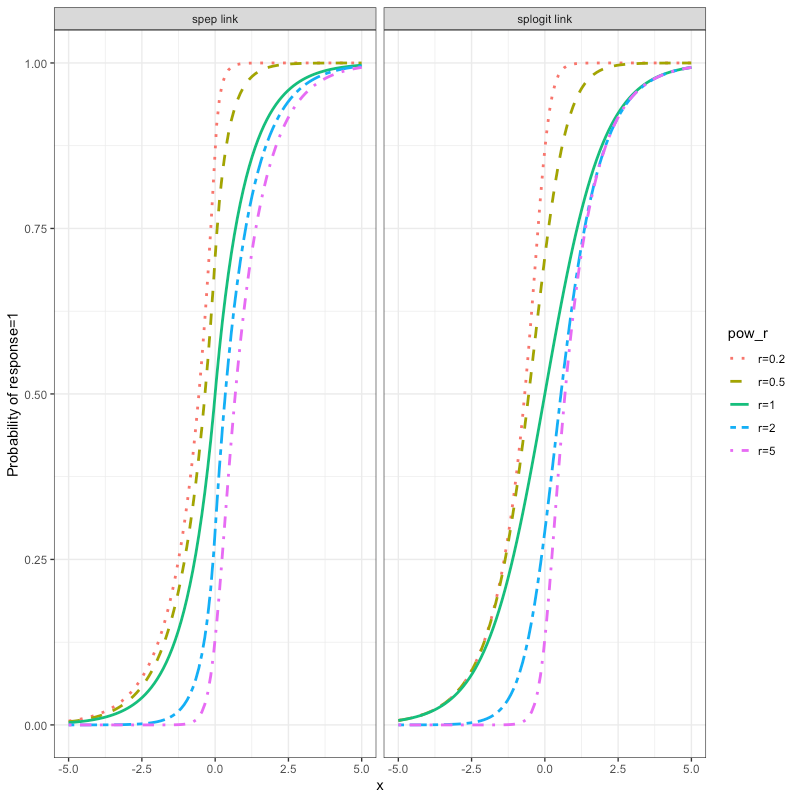
\includegraphics[width=0.9\textwidth]{Figures/Chp2_cdf_sp.png}
\caption{Plot for $F_{\mbox{splogit}}$ and $F_{\mbox{spep}}$}
\label{fig:Chp2_cdf_sp}
\end{figure}

\subsection{Prior Specifications and Posterior Inference}\label{sec:chp2_prior}

For all unknown parameters, we assume the following prior distributions: 1) regression coefficients $(\bm{\alpha}^T, \bm{\beta}^T$): non-informative multivariate normal priors with mean $\bm{0}$ and a large variance; 2) scale parameters $(\sigma_b,\sigma_u,\sigma)$: weakly informative proper priors with half Cauchy distribution \cite{Gelman2006}; 3) correlation scale parameter $\tau$: a truncated normal distribution; 4) correlation length-scale parameter $\rho$: a diffuse inverse gamma prior; 5) power parameters $\bm{r}^T$: gamma distributions \cite{Jiang2013}$,$ \cite{Upadhyay2015}; 6) association parameters $(\rho_1, \rho_2)$: uniform priors. Explicit values of hyperparameters are included in Appendix \ref{app:b}.

Let $\bm{\Psi}=(\bm{\alpha}^T, \bm{\beta}^T, \bm{r}^T,\sigma_b,\sigma_u,\sigma,\tau,\rho,\rho_1,\rho_2)$, $\bm{D}_{obs}=(\bm{Y}_{li},\bm{R}_{li})^T$, the joint posterior distribution of $(\bm{\Psi},\bm{b},\bm{U},\bm{W})$ is written as 

\begin{equation}
\begin{split}
\pi(\bm{\Psi},\bm{b},\bm{U},\bm{W}|\bm{D}_{obs}) \propto &
  \pi(\bm{D}_{obs},\bm{b},\bm{U},\bm{W}|\bm{\Psi}) \pi(\bm{\Psi}) \\
\propto & \pi(\bm{D}_{obs}|\bm{b},\bm{U},\bm{W},\bm{\Psi}) \pi(\bm{b}|\bm{U},\bm{W},\bm{\Psi})\pi(\bm{U}|\bm{W},\bm{\Psi}) \pi(\bm{W}|\bm{\Psi})\pi(\bm{\Psi}) \\ 
 \propto & \pi(\bm{Y},\bm{R}|\bm{b},\bm{U},\bm{W},\bm{\Psi}) \pi(\bm{b}|\bm{\Psi}) \pi(\bm{U}|\bm{\Psi}) \pi(\bm{W}|\bm{\Psi}) \pi(\bm{\Psi}) \\
 \propto & \prod_{l=1}^{L}\prod_{i=1}^{n_l}I(\bm{Y}_{li},\bm{R}_{li}|b_{l}, U_{li}, \bm{W}_{li}, \bm{\Psi}) \pi(b_l|\sigma_b) \pi(U_{li}|\sigma_u) \pi(\bm{W}_{li}|\tau,\rho) \pi(\bm{\Psi})
\end{split}
\end{equation}
where the likelihood function $\bm{I}(\bm{Y}_{li},\bm{R}_{li}|b_l,U_{li},\bm{W}_{li},\bm{\Psi})= \bm{I}_1(\bm{Y}_{li}|b_l,U_{li},\bm{W}_{li},\bm{\Psi}) \bm{I}_2(\bm{R}_{li}|b_l,U_{li},\bm{\Psi})$ by the assumption of conditional independence between $\bm{Y}$ and $\bm{R}$ given random effects $\bm{b}$ and $\bm{U}$. We further suppress the dependence of each component in $\bm{\Psi}$.

% All posterior samplings are carried out through HMC by R interface to Stan, namely RStan \cite{Rstan2020}.

\subsection{Dynamic Individual Prediction} \label{sec:chp2_pred}

We employ the best linear unbiased predictor (BLUP) to predict individual random intercept $U_{li'}$ and time-continuous random variable $\bm{W}_{li'}(t)$ for any new patient $i'$ from the existing center $l$. The explicit forms are obtained by the properties of the multivariate normal distribution as utilized in \cite{Diggle2015} as 

\begin{align}
    E\big(U_{li'}|\bm{Y}_{li'},b_l, \bm{\phi},\bm{\alpha}\big)  = & \sigma_u^2\bm{K}^T_{li'}\big(\bm{V}_{li'}(\bm{\phi})\big)^{-1} (\bm{Y}_{li'}-\bm{X}_{li'}\bm{\alpha}-b_l\bm{K}_{li'})\label{chp2:eq4} \\
    E\big(W_{li'}(t_{li'j}\big)|\bm{Y}_{li'},b_l, \bm{\phi},\bm{\alpha})  =  & \tau^2\bm{F}^{j^T}_{li'}\big(\bm{V}^j_{li'}(\bm{\phi})\big)^{-1}  (\bm{Y}^j_{li'}-\bm{X}^{j}_{li'}\bm{\alpha}-b_l\bm{K}^j_{li'}) \label{chp2:eq5}
\end{align}
where $\bm{Y}_{li'}$ and $\bm{X}_{li'}$ are observed data and covariates, respectively. $\bm{K}_{li'}$ denotes an $n_{li'} \times 1$ matrix of ones and $\bm{\alpha}$ is as before. Also,
 
 \begin{equation}
    \bm{V}_{li'}(\bm{\phi})=\sigma_u^2\bm{J}_{li'}+\tau^2\bm{R}_{li'}+\sigma^2\bm{I}_{li'}
 \end{equation} 
 where $\bm{\phi}=(\sigma^2_2,\tau^2,\sigma^2,\rho)$, $\bm{J}_{li'}$ is an $n_{li'} \times n_{li'}$ matrix of ones, $\bm{R}_{li'}$ is an $n_{li'} \times n_{li'}$ matrix with $(t,t')th$ element $exp(-|t-t'| \cdot \rho)$ and $\bm{I}_{li'}$ is an $n_{li'} \times n_{li'}$ identity matrix.
 
 Let response and covariates history up to an observed time point $j$ be presented by $\bm{Y}_{li'}^j$ and  $\bm{X}_{li'}^j$ in Equation (\ref{chp2:eq5}). $\bm{F}^j_{li'}=\Big(exp(-|t_{li'1}-t_{li'j}| \cdot \rho), \dots, exp(-|t_{li'j}-t_{li'j}| \cdot \rho) \Big)^T$, $\bm{V}^j_{li'}$ is the variance-covariance matrix of $\bm{Y}^j_{li'}$. Analogously, forecasting $W_{lij'}$ at time $t_{lij}$ with lead-time $u$ for an existing patient $i$ is obtained by 
 \begin{equation}
  E\big(W_{li}(t_{lij}+u)|\bm{Y}^j_{li},b_l, U_{li},\bm{\phi}, \bm{\alpha}\big)  =  \tau^2\bm{F}^{{j,u}^T}_{li}\big(\bm{G}^j_{li}(\bm{\phi})\big)^{-1}(\bm{Y}^j_{li}-\bm{X}^{j}_{li}\bm{\alpha}-b_l\bm{K}^j_{li}-U_{li}\bm{K}^j_{li}) \label{chp2:eq6}
\end{equation}
where $\bm{G}^j_{li}(\bm{\phi})=\tau^2\bm{R}^j_{li}+\sigma^2\bm{I}^j_{li}$, $\bm{R}^j_{li}$ and $\bm{I}^j_{li}$ are as before but with new dimensions of $j \times j$. $\bm{F}^{j,u}_{li}=\Big(exp(-|t_{lij}+u-t_{li1}| \cdot \rho),\dots,exp(-|t_{lij}+u-t_{lij}| \cdot \rho) \Big)^T$. Whenever a new response at time $t_{lij'}$ becomes available, the prediction from Equation (\ref{chp2:eq6}) will be dynamically updated. 
In the real data study, we apply empirical BLUPs to achieve the prognosis for ppFEV1 and PE according to Equation \ref{eq:chp2_jm}. 

% \begin{align*}
% & \mbox{Predict for new patients} \left \{\begin{array}{ll}
%  E({Y}_{li'j}) = \bm{X}_{li'}(t_{li'j})\widehat{\bm{\alpha}}+\widehat{\rho}_1\widehat{b}_l+\widehat{\rho}_2\widehat{U}_{li'}+\widehat{W}_{li'}(t_{li'j})\\
%  Pr(R_{li'j}=1) = F_{sp}\big(\bm{V}_{li}(t_{li'j})\widehat{\bm{\beta}}+\widehat{\rho}_1\widehat{b}_l+\hat{\rho}_2\widehat{U}_{li'};\widehat{r}_l\big)
% \end{array}\right. \\\\
% & \mbox{Forecast for existing patients} \left \{\begin{array}{ll}
%  E({Y}_{lij'})  = \bm{X}_{li}(t_{lij'})\widehat{\bm{\alpha}}+\widehat{\rho}_1\widehat{b}_l+\widehat{\rho}_2\widehat{U}_{li}+\widehat{W}_{li}(t_{lij'})\\
%  Pr(R_{lij'}=1)  = F_{sp}\big(\bm{V}_{li}(t_{lij'})\widehat{\bm{\beta}}+\widehat{\rho}_1\widehat{b}_l+\widehat{\rho}_2\widehat{U}_{li};\widehat{r}_l\big)
% \end{array}\right.
% \end{align*}

\subsection{Model Selection}

In this section we consider a recent measure of comparison between models. The Watanabe-Akaike information criterion (WAIC) \cite{Watanabe2010} is favored as a full Bayesian approach for estimating the out-of-sample expectation, by averaging over the posterior distribution rather than conditioning on a point estimate, thus is invariant to reparameterisations contrary to the Deviance Information Criterion (DIC) \cite{Spiegelhalter2002}. In a comprehensive review paper, Gelman and his colleagues \cite{Gelman2014} recommended expression on the deviance scale in terms of variance adjustment, written as

\begin{equation}
    \begin{split}
    \mbox{WAIC}=-2\Big \{\sum_{i=1}^{n}log\big(p_{post}(y_i|\theta)\big)-\sum_{i=1}^{n}\mbox{var} \Big (log\big( p_{post}(y_i|\theta)\big) \Big ) \Big \}
    \end{split}
\end{equation}

Computed $\mbox{WAIC}_1$ and $\mbox{WAIC}_2$ for the two submodels are defined as follows

\begin{align}
  & \widehat{\mbox{WAIC}}_1=-2\Big \{\sum^{L}_{l=1}\sum^{n_l}_{i=1}\sum^{n_{li}}_{j=1}\Big ( log\big [\frac{1}{S}\sum_{s=1}^S \bm{I}_1(Y_{lij}|b^s_l,U^s_{li},W^s_{lij},\bm{\Psi}^s)\big] - V_{s=1}^{S}log\big[\bm{I}_1(Y_{lij}|b^s_l,U^s_{li},W^s_{lij}, \bm{\Psi}^s)\big] \Big ) \Big \} \label{eq:waic1}\\   
  & \widehat{\mbox{WAIC}}_2=-2\Big \{\sum^{L}_{l=1}\sum^{n_l}_{i=1}\sum^{n_{li}}_{j=1}\Big (log\big [\frac{1}{S}\sum_{s=1}^S \bm{I}_2(R_{lij}|b^s_l,U^s_{li},\bm{\Psi}^s)\big] -  V_{s=1}^{S}log\big[\bm{I}_2(R_{lij}|b^s_l,U^s_{li}, \bm{\Psi}^s)\big] \Big ) \Big \}  \label{eq:waic2}
\end{align}
where $\bm{I}_1$ and $\bm{I}_2$ denote the likelihood function for normal distribution and bernoulli distribution, respectively. $S$ is the number of simulation draws, $\bm{\Psi}^s$ is the vector of the model parameters at $s^{th}$ iteration. $V_{s=1}^S$ represents the sample variance, that is $V_{s=1}^S\bm{a}=\frac{1}{S-1}\Sigma^{S}_{s=1}(a_s-\bar{a})^2$. Practically, calculations on Equation (\ref{eq:waic1}) and (\ref{eq:waic2}) could be easily achieved by the \emph{waic} function from the \emph{loo} package (v2.3.1) \cite{Vehtari2020} by extracting pointwise log-likelihood values from the posterior samplings. The model with the smaller WAIC indicates the better goodness of fit. 

\section{Simulated Examples} \label{sec:chp2_sim}

\subsection{Simulation Study A}

The first simulation study is designed to explore the flexibility of splogit in comparison with three common links, namely logit, probit, cloglog. Hereafter, we name them by the rule of link-JM. The explicit expressions are shown as

\begin{align}
& \left \{\begin{array}{ll}
  F_{\mbox{splogit}}(x)= [1+exp(\frac{x}{r})]^{-r}I_{(0,1]}(r)+\big\{1-[1+exp(-rx)]^{-\frac{1}{r}}\big\} I_{(1,+\infty)}(r)\\ 
  F_{\mbox{logit}}(x)= [1+exp(x)]^{-1}\\ 
  F_{\mbox{probit}}(x)= \Phi(x), \mbox{where $\Phi$ is the cdf of standard normal }\\ 
  F_{\mbox{cloglog}}(x)= 1-e^{-e^x}
\end{array}\right.
\end{align}
Then we simulate multicenter data sets with proposed splogit-JM to fit following joint models, of the forms

\begin{align*}
\mbox{logit-JM} & \left \{\begin{array}{ll}
        Y_{lij}= \alpha_0 + x_{li1}\alpha_1 + x_{li2}\alpha_2 + b_l + U_{li} + \epsilon_{lij} \\
       \mbox{Pr}(R_{lij}=1)=F_{\mbox{logit}}(\beta_0 + \beta_1 t_{lij} + \rho_1 b_l + \rho_2 U_{li}) \\
\end{array}\right. \\
\mbox{probit-JM} & \left \{\begin{array}{ll}
       Y_{lij}= \alpha_0 + x_{li1}\alpha_1 + x_{li2}\alpha_1+b_l+U_{li} + \epsilon_{lij} \\
       \mbox{Pr}(R_{lij}=1)=F_{\mbox{probit}}(\beta_0 + \beta_1 t_{lij} +\rho_1 b_l + \rho_2 U_{li}) \\
\end{array}\right. \\
\mbox{cloglog-JM} & \left \{\begin{array}{ll}
       Y_{lij}= \alpha_0 + x_{li1}\alpha_1 + x_{li2}\alpha_1+b_l+U_{li} + \epsilon_{lij} \\
       \mbox{Pr}(R_{lij}=1)=F_{\mbox{cloglog}}(\beta_0 + \beta_1 t_{lij} + \rho_1 b_l + \rho_2 U_{li}) \\
        \end{array}\right.\\
\mbox{splogit-JM} & \left \{\begin{array}{ll}
       Y_{lij}= \alpha_0 + x_{li1}\alpha_1 + x_{li2}\alpha_1+b_l+U_{li} + \epsilon_{lij} \\
       \mbox{Pr}(R_{lij}=1)=F_{\mbox{splogit}}(\beta_0 + \beta_1 t_{lij} + \rho_1 b_l + \rho_2 U_{li};r_l) \\
       \end{array}\right.        
\end{align*}
where all the notations are as before. Without loss of generality, we simulate a balanced data set, that is $L=5,n_l=50, n_{li}=5$ for 50 replicates. Moreover, we set regression coefficients $\alpha_0=1, \alpha_1=-3, \alpha_2=0.7, \beta_0=0.5, \beta_1=4$, power parameter $\bm{r}=(0.2, 0.5, 1, 2, 3)^T$ and association parameters $\rho_1=0.5, \rho_2=0.8$. Let $x_{li1} \sim N(0,1), x_{li2} \sim \mbox{Bernoulli}(0.5), b_l \sim N(0,\sigma^2_b), U_{li} \sim N(0,\sigma^2_u)$ and $\epsilon_{lij} \sim N(0, \sigma^2)$, with $\sigma_b=5, \sigma_u=3, \sigma=0.45$. Time point $t_{lij}$ is simulated from a uniform(0,6) distribution by assuming every patient starts from time=0 and is standardized to ensure the computational stability.  

All models are estimated by HMC with 4000 post-warmup iterations via two chains. Averaged results and model information criterion are summarized in Figure \ref{fig:chp2_sima} and Table \ref{tab:chp2_sima}, respectively. Posterior samplings are ensured to converge until all values for the potential scale reduction factor $\hat{R}$ are below 1.1 (\cite{Gelman1992}). All other details can be found in Appendix \ref{app:b}. 

\begin{center}
\begin{table}[H]
\caption{Comparison of logit-, probit-, cloglog- and splogit-JM over simulated data sets for 50 replicates}
\label{tab:chp2_sima}
 \centering
 \begin{threeparttable}
  \begin{tabular}{m{0.2\textwidth}m{0.2\textwidth}m{0.2\textwidth}m{0.2\textwidth}}
  \toprule
 Fitted Model & $\mbox{WAIC}$ \tnote{a} \hspace*{1.8mm} & $\mbox{WAIC}_1$ \tnote{b}  \hspace*{1.8mm}  & $\mbox{WAIC}_2$ \tnote{c}  \hspace*{1.8mm}\\
 \midrule
   logit-JM & 2239.93 & 1807.16 & 432.77 \\
  
   probit-JM & 2244.44 & 1807.49 & 436.95 \\
  
   cloglog-JM & 2272.57  & 1808.24 & 464.33 \\
   
   \bf splogit-JM & 2203.00 & 1806.37 & 396.63 \\
    \bottomrule
  \end{tabular}
   \begin{tablenotes}[para]
    \footnotesize
    Note: model in boldface: true model; \item[a] Joint model; \item[b] Continuous submodel; \item[c] Binary submodel
    \end{tablenotes}
    \end{threeparttable}
\end{table}
\end{center}

\begin{figure}[H]
\centering
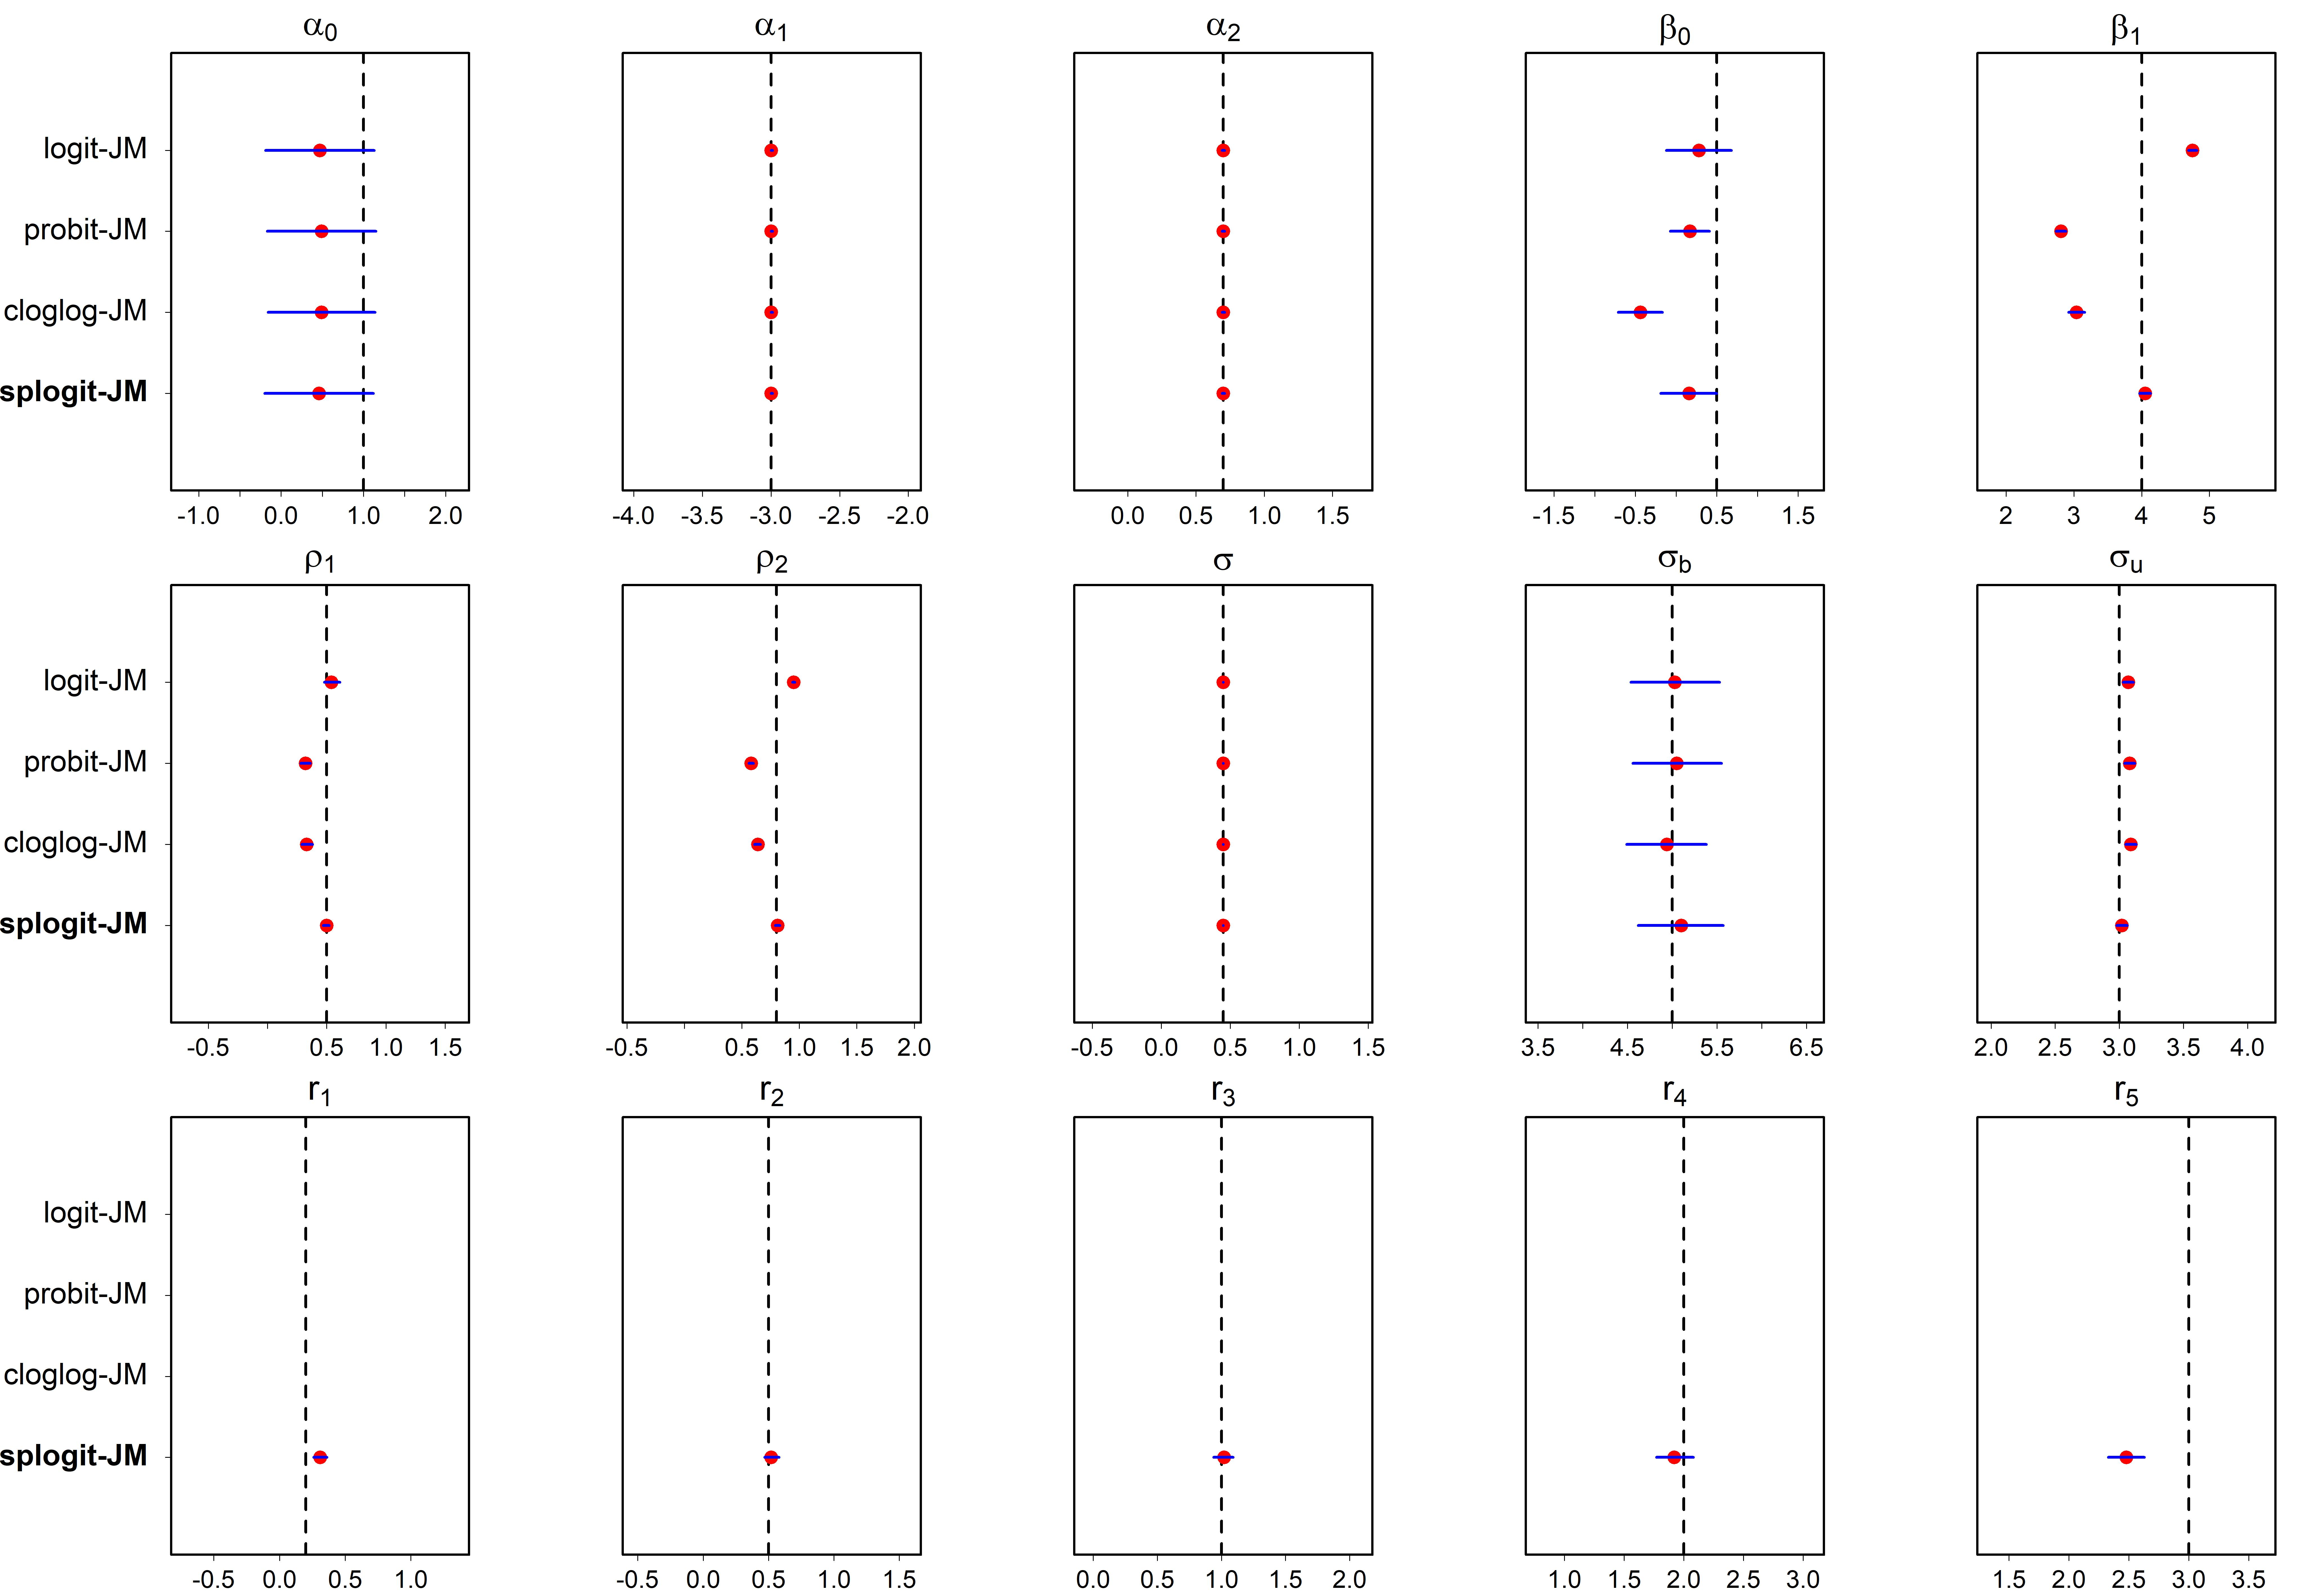
\includegraphics[width=\textwidth]{Figures/Chp2_SIM_SPLOGIT_A.jpg}
\caption{Averaged posterior means by 50 replicates via CmdStanr with true model (boldface), true value (dashed vertical line), posterior mean estimates (red dot) and corresponding 95\% confidence interval (blue line).}
\label{fig:chp2_sima}
\end{figure}

Table \ref{tab:chp2_sima} demonstrates that center-specific power parameter induces great flexibility than common fixed links in a hierarchical data structure by the smallest $\mbox{WAIC}_2$. Among those conventional links, logit-JM as the special case of true splogit-JM outperforms others. Figure \ref{fig:chp2_sima} shows the reasonable performance in recovering the true values (especially $\sigma_b$) and we concur that estimates for $\alpha_0$ and $r_5$ can be further improved with more iterations or sample size or replicates.   

\subsection{Simulation Study B} 

In this section, we implement another simulation study to explore the performance of JM under eight scenarios (four JMs $\times$ two flexible links). We take the LME submodel without fixed effects for simplicity purpose and JM equations are specified as follows 
\begin{align*}
& \mbox{JM}_1 \left \{\begin{array}{ll}
        Y_{lij}= U_{li} + \epsilon_{lij} \\
       \mbox{Pr}(R_{lij}=1)=F_{sp}(\beta_0+\beta_1t_{lij}+ \rho_2 U_{li};r) \\
\end{array}\right. \\
& \mbox{JM}_2 \left \{\begin{array}{ll}
        Y_{lij}=b_l + U_{li} + \epsilon_{lij}\\
       \mbox{Pr}(R_{lij}=1)=F_{sp}(\beta_0+\beta_1t_{lij}+\rho_1 b_l + \rho_2 U_{li};r) \\
\end{array}\right. \\
&\mbox{JM}_3 \left \{\begin{array}{ll}
       Y_{lij}=b_l + U_{li} + \epsilon_{lij} \\
       \mbox{Pr}(R_{lij}=1)=F_{sp}(\beta_0+\beta_1t_{lij}+\rho_1 b_l + \rho_2 U_{li};r_l) \\
        \end{array}\right.\\
&\mbox{JM}_4 \left \{\begin{array}{ll}
        Y_{lij}=b_l + U_{li} + W_{lij} + \epsilon_{lij} \\
       \mbox{Pr}(R_{lij}=1)=F_{sp}(\beta_0+\beta_1t_{lij}+\rho_1 b_l + \rho_2 U_{li};r_l) \\
       \end{array}\right.        
\end{align*}
where $\mbox{JM}_1$ is designed as a misspecified model and $\mbox{JM}_4$ is the proposed model with exponential correlation and center-specific power parameter; $t_{lij}$ is a standardized age variable for the stabilization of posterior computations. We set regression coefficients $\beta_0=0.5$, $\beta_1=4$ and association parameters $\rho_1=0.5$, $\rho_2=0.8$. Let $b_l \sim N(0,\sigma^2_b)$, $U_{li} \sim N(0,\sigma^2_u)$ and $\epsilon_{lij} \sim N(0,\sigma^2)$, with $l=1, \dots,5, i=1, \dots, 50, j=1, \dots, 10, \sigma_b=5, \sigma_u=3, \sigma=0.45$; $W_{li}(\bm{t})$ be the stationary Gaussian process with $\tau=1.5$ and $\rho=0.5$ as defined in Section \ref{eq:chp2_w}. We simulate a total of 100 data sets (50 for splogit-$\mbox{JM}_4$ and 50 for spep-$\mbox{JM}_4$) under true power parameters $\bm{r}=(0.2, 0.5, 1, 1, 2)^T$. Priors are defined according to Section \ref{sec:chp2_prior}. All models are estimated by HMC with at least 10,000 iterations via two chains. The first 4000 draws are discarded as a warm-up sampling and every third values are kept for the posterior inference. We ensure all results satisfy the convergence diagnostic $\hat{R}$.

\begin{center}
\begin{table}[ht]
\caption{Model comparisons over simulated data sets for 50 replicates} \label{tab:chp2_sim}
 \centering
 \begin{threeparttable}
  \begin{tabular}{lllllll}
    \toprule
   & \multicolumn{6}{c} {True Model}\\
    \cmidrule(lr) {2-7} 
  Fitted Model & \multicolumn{3}{c}{splogit-$\mbox{JM}_4$} & \multicolumn{3}{c}{spep-$\mbox{JM}_4$}  \\
 \cmidrule(lr) {2-4}  \cmidrule(lr) {5-7}
 & $\mbox{WAIC} \tnote{a} $ & $\mbox{WAIC}_1 \tnote{b}$  & $\mbox{WAIC}_2 \tnote{c}$  &
 $\mbox{WAIC} \tnote{a}$ & $\mbox{WAIC}_1 \tnote{b}$ & $\mbox{WAIC}_2 \tnote{c}$ \\
 \midrule 
   Misspecified ($\mbox{JM}_1$) & 9455.853 & 8369.268 & 1086.585 &
                9256.9877 & 8299.09 & 957.8977 \\
  
   No center-index ($\mbox{JM}_2$) & 9362.319 & 8360.999 & 1001.32 &
                9179.9247 &  8292.143 &  887.7817 \\
  
   No covariance ($\mbox{JM}_3$) &  9328.3859 & 8360.075 & 968.3109 &
                 9157.4637 & 8291.87 &  865.5937 \\
   
   \textbf{Proposed ($\mbox{JM}_4$)} & \textbf{8508.9091} & \textbf{7574.098} & \textbf{934.8111} & \textbf{8352.8335} & \textbf{7541.872} & \textbf{810.9615} \\
    \bottomrule
  \end{tabular}
   \begin{tablenotes}[para]
    \footnotesize
        Note: model in boldface: true model; value in boldface: the smallest value; \item[a] Joint model; \item[b] Continuous submodel; \item[c] Binary submodel
    \end{tablenotes}
    \end{threeparttable}
\end {table}
\end{center}

As shown in Table \ref{tab:chp2_sim}, both splogit-$\mbox{JM}_4$ and spep-$\mbox{JM}_4$ are correctly identified by the lowest WAIC, while both splogit-$\mbox{JM}_1$ and spep-$\mbox{JM}_1$ perform the worst, reflecting that ignoring center effect in a multicenter cohort study yields poor performance. Figure \ref{fig:chp2_simb1} and \ref{fig:chp2_simb2} illustrate that posterior mean estimates of the true joint model have negligible bias, indicating that the proposed joint model provide valid Bayesian inference. The striking biases from all other three joint models are found from scale parameter ($\sigma$) for the measurement error. In addition, we note that misspecified joint model produces misleading results for standard deviation parameter $\sigma_u$, which might result in improper inference.

% We summarize the posterior mean with 95\% credible interval for each parameter with the resulting 2000 iterations in Appendix \ref{app:b}. 

\begin{figure}[ht]
\centering
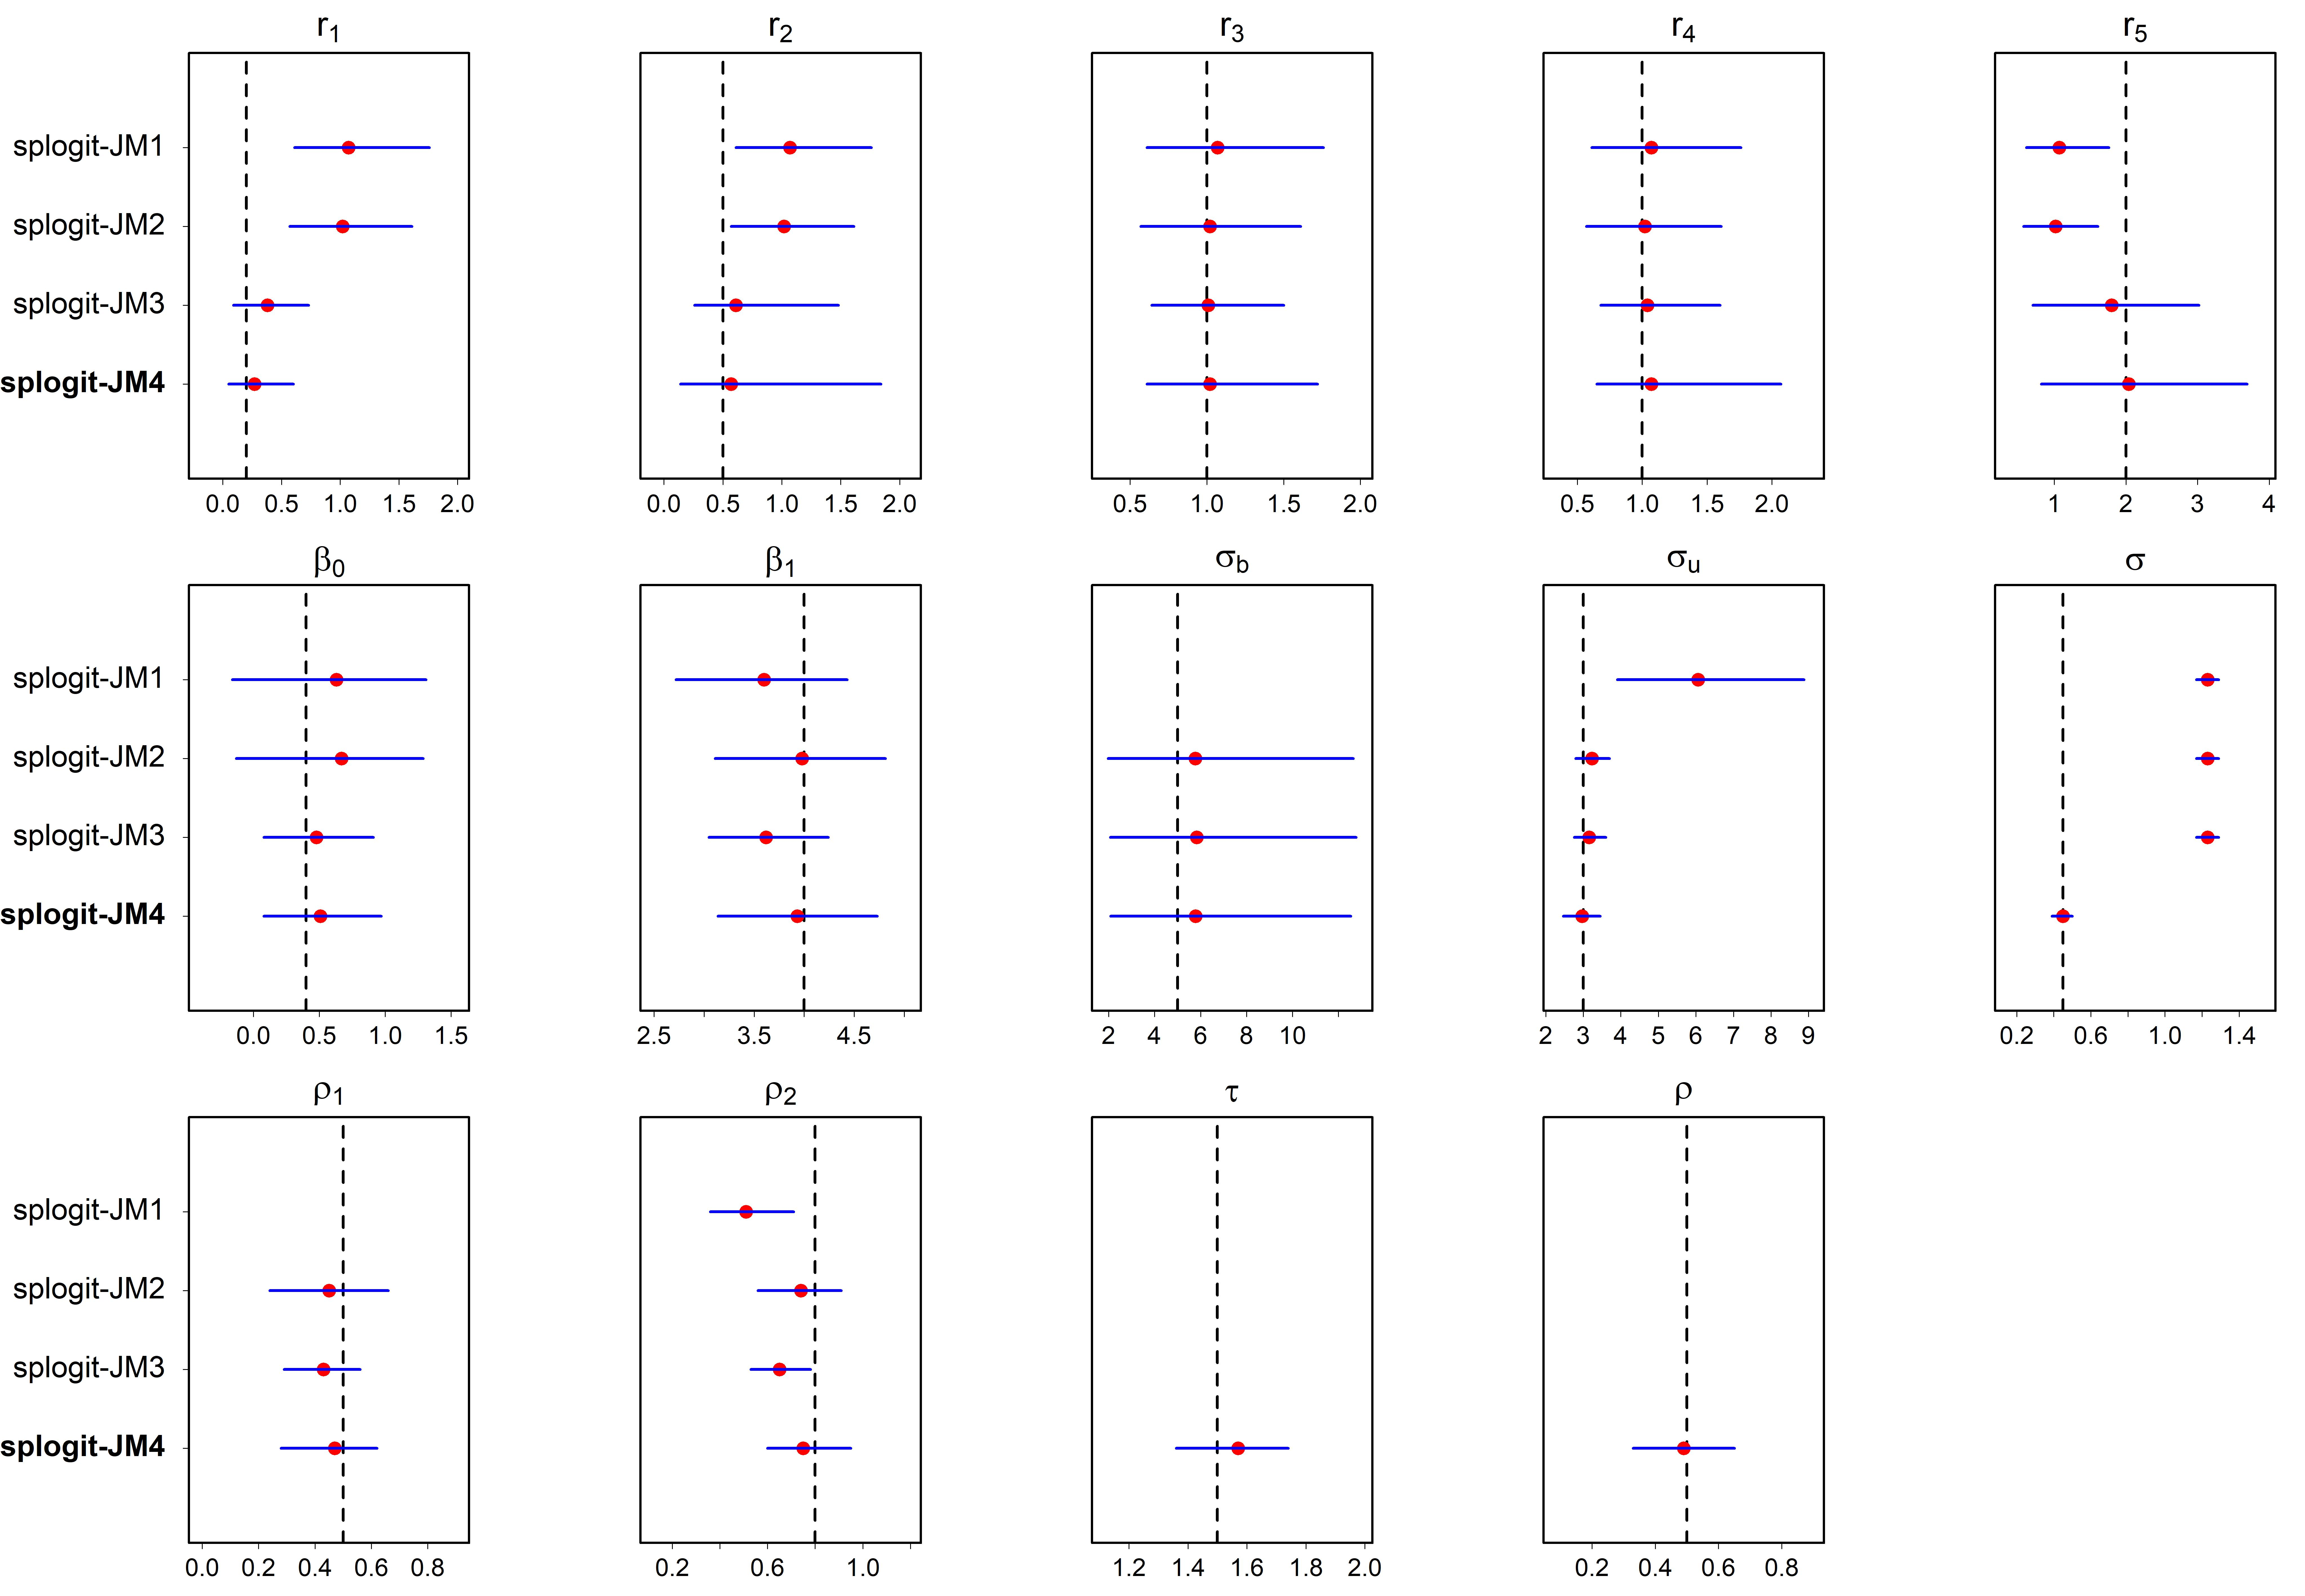
\includegraphics[width=\textwidth]{Figures/Chp2_SIM_SPLOGIT_B.jpg}
\caption{Averaged posterior means by 50 replicates via RStan with true model (boldface),  rue value (dashed vertical line), posterior mean estimates (red dot) and corresponding 95\% credible interval (blue line). JM1: Misspecified JM; JM2: No center-index JM; JM3: No covariance JM. }
\label{fig:chp2_simb1}
\end{figure}


\begin{figure}[ht]
\centering
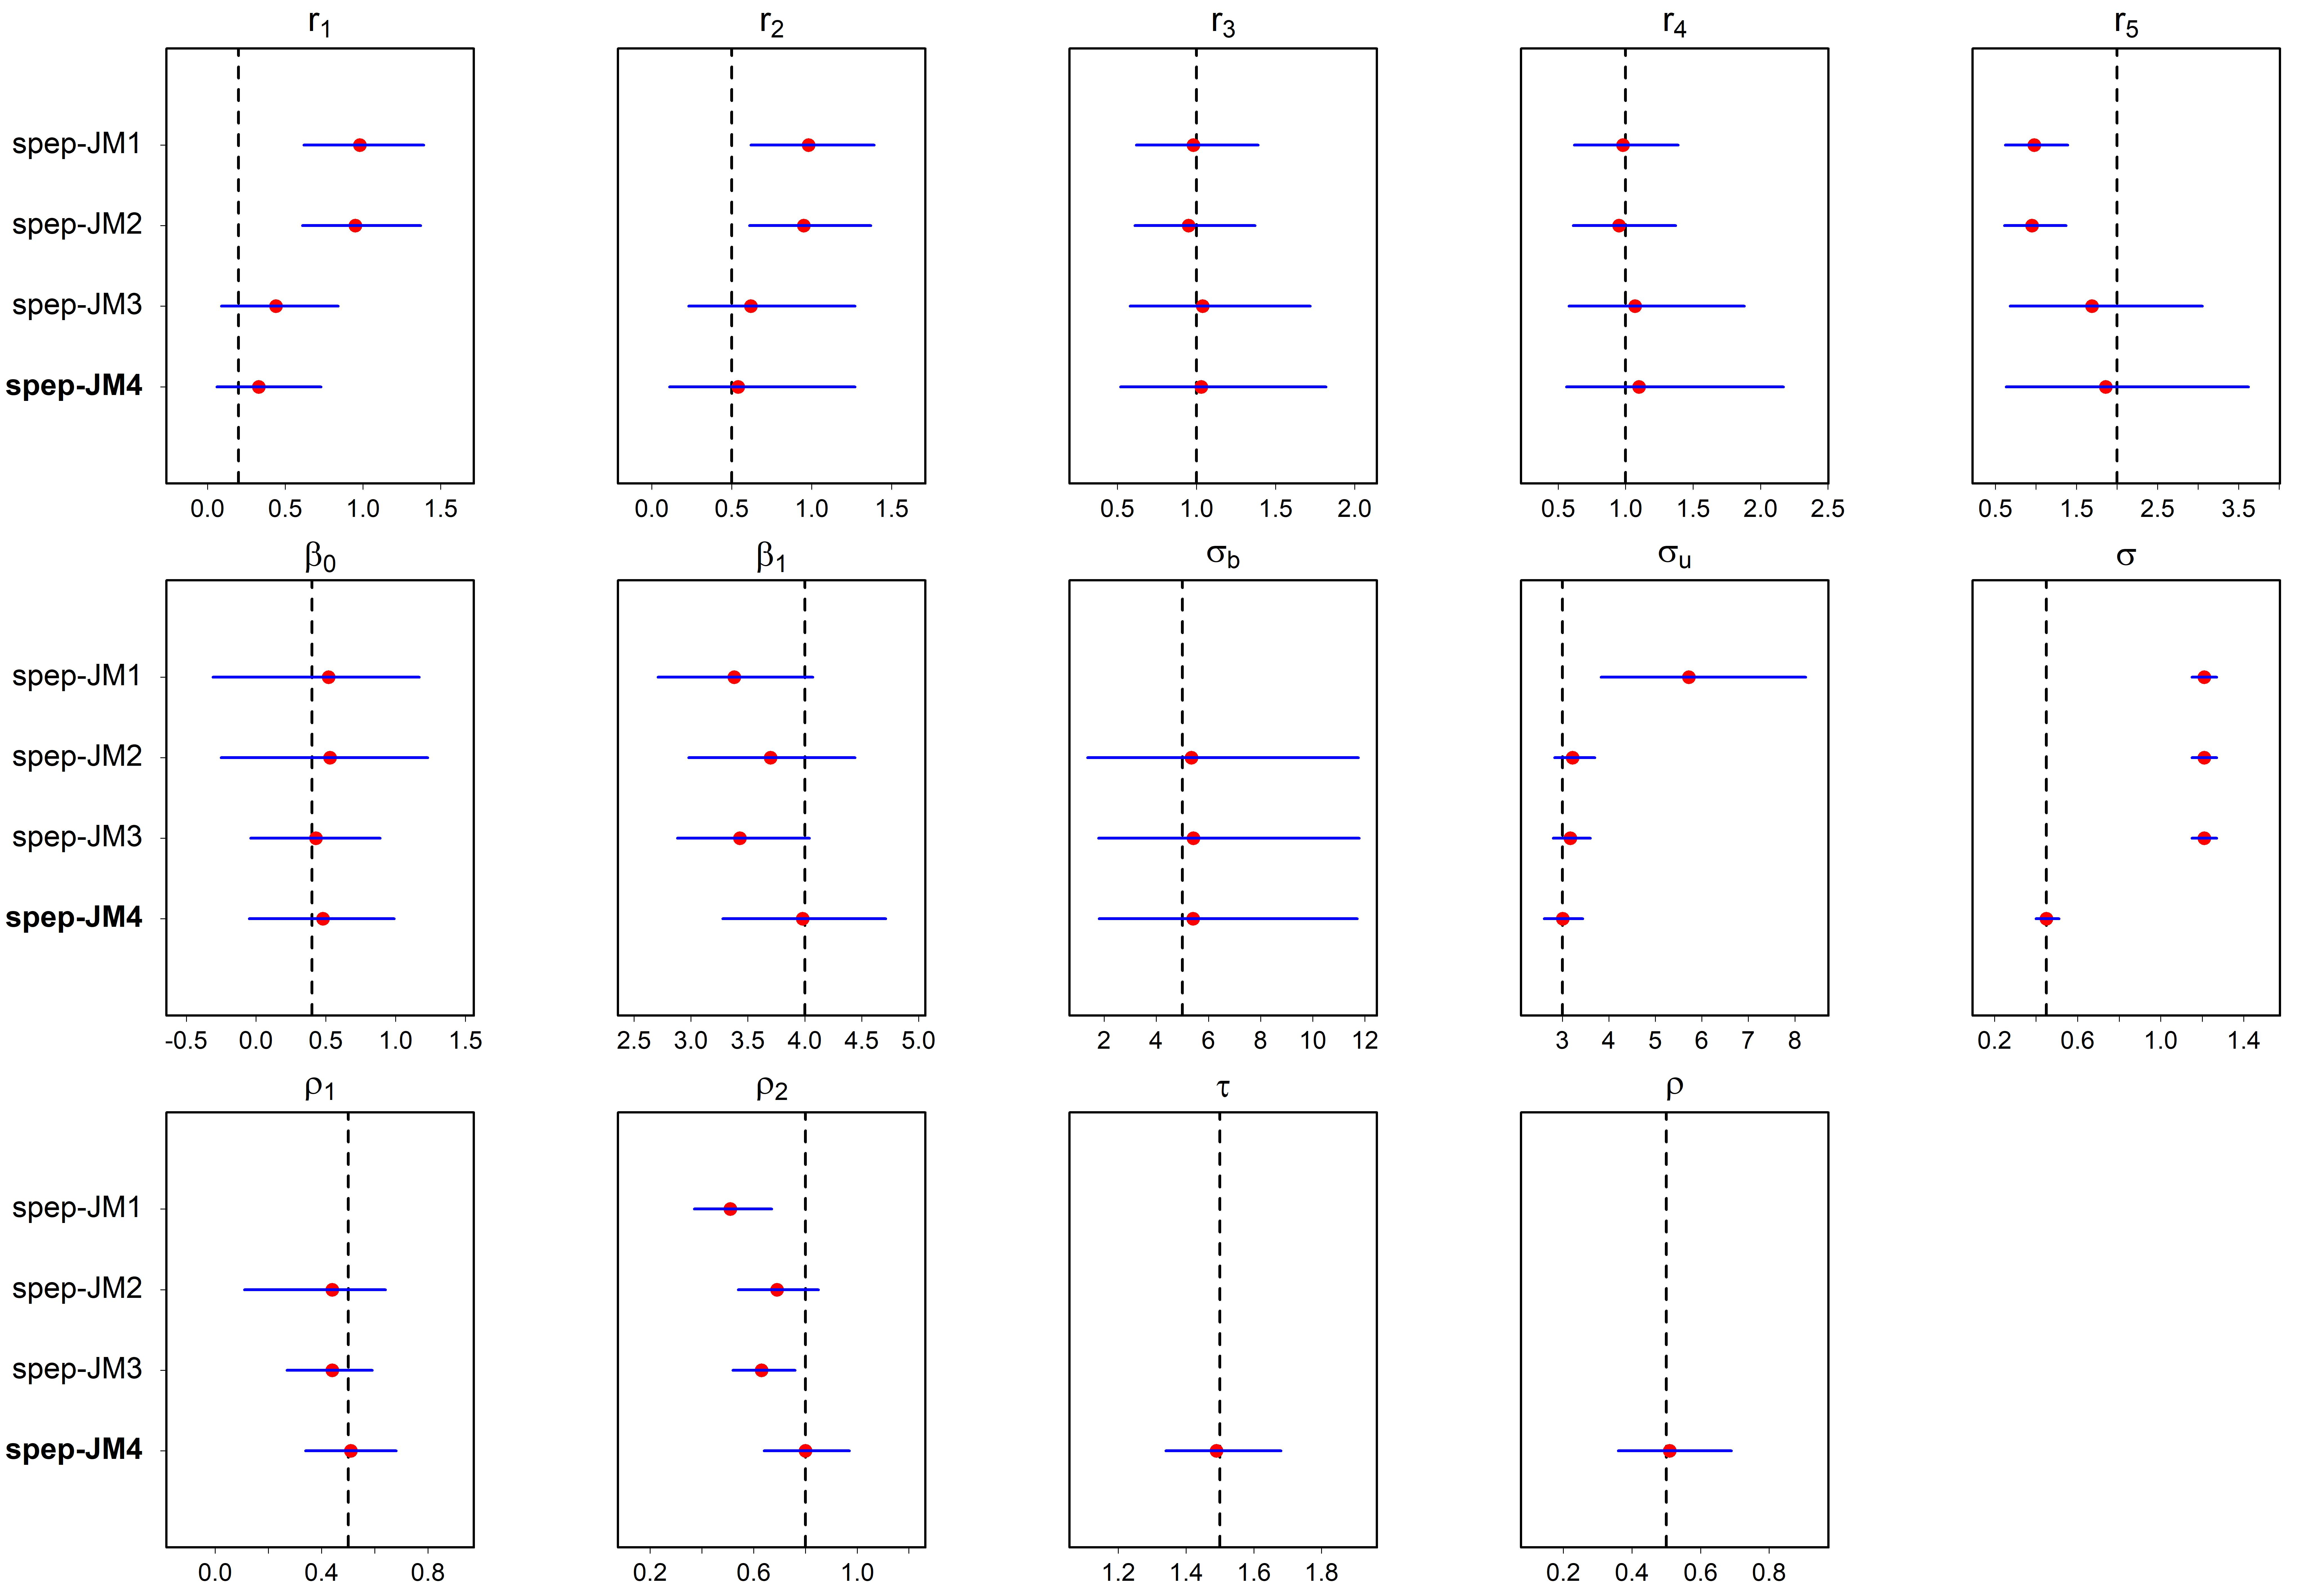
\includegraphics[width=\textwidth]{Figures/Chp2_SIM_SPEP_B.jpg}
\caption{Averaged posterior means by 50 replicates via RStan with true model (boldface),  rue value (dashed vertical line), posterior mean estimates (red dot) and corresponding 95\% credible interval (blue line). JM1: Misspecified JM; JM2: No center-index JM; JM3: No covariance JM. }
\label{fig:chp2_simb2}
\end{figure}

\section{Application} \label{sec:chp2_app}

\subsection{Motivating Data}
Our analysis cohort for this application consists of 381 CF patients who contributed a total of 9,209 observations across five centers. These centers are randomly selected among those with feasible sample size between 50 and 100 for computational aspects of the modeling. Around 15\% of measurements are excluded due to missing values on ppFEV1 and Body Mass Index (BMI). We observe neither drop-outs (e.g. death or lung transplantation) nor patients switch centers during the observed period. Data cleaning and descriptive statistics are summarized in Appendix \ref{app:b}. Approval for the data analysis was made by the Institutional Review Boards from Cincinnati Children's Hospital Medical Center and University of Cincinnati. 

\begin{figure}[ht]
\centering
\includegraphics[width=\textwidth]{Figures/Chp2_display.jpg}
\caption{Observed ppFEV1 (left panel) and density of PE (right panel) against time since the first PE occurrence. Within each longitudinal plot: three randomly selected patient profiles (solid black lines), observed values (gray dots), and center-specific LOWESS smoothing curves with 95\% confidence interval (blue solid lines with gray-shaded bands); Within each density plot: histograms (bars) with densities (areas) grouped by PE occurrence; Abbreviation: Freq. = frequency}
\label{display}
\end{figure}

We restrict encounter age to include observations taken under valid pulmonary function testing (above 6 years old) and up to early adolescence (12 years old). The upper limit is chosen to restrict the cohort to the first bout of lung function decline, which is shown to occur before more rapid decline during late adolescence and early adulthood \cite{Szczesniak2014}. To be included in the analysis, patients should have at least three or more observed ppFEV1 measurements spanning at least six months after the first PE occurrence. The time period selected for this analysis is from calendar year 2003 to 2017, because modern predictors with encounter levels are consistently documented beginning in 2003 \cite{Knapp2016}. Average (range) duration of follow-up is 4.08 (0.53-5.99) years. Figure \ref{display} displays trajectories of ppFEV1 and densities of PE throughout the whole analysis period. The left panel demonstrates the heterogeneous nature of ppFEV1 with a slightly increasing, smoothing curve in each center. The right panel indicates some underlying skewness of PE responses. 

\subsection{Internal Validation}

To access the predictive performance, we conduct 80-20\% cross-validation by choosing a random sample of 20\% of patients from each center, in which 79 patients with 1993 observations are for testing cohort. Among those remaining 80\% patients, we select the first 80\% observations with at least three records spanning at least six months after the first PE for the training cohort, which consists of 302 patients with 5769 observations and the rest of their 1447 observations are conformed as the masking cohort.

\subsection{Model Estimation}

Predictors are selected by a conventional \emph{Stepwise} method (\cite{Hocking1976}) from a two-stage model basis. We apply the R function \emph{buildlme} from \emph{buildmer} package \cite{buildmer2021} for LME submodel and the R function \emph{step} from \emph{stats} package \cite{R2020} for GLMM. By defining the baseline as the time of the first PE event, we finally include baseline ppFEV1, BMI percentile, Methicillin-resistant Staphylococcus aureus (MRSA), pseudomonas aeruginosa (pa) and genotype F508del heterozygote for the LME submodel; time since baseline (in years), BMI percentile, pancreatic enzyme usage and pa for the GLMM.

\begin{center}
\begin{table}[H]
 \caption{Model comparisons for CF data with the boldface as the preferred model.} \label{tab:chp2_app_waic}
 \centering
   \begin{threeparttable}
  \begin{tabular}{m{0.3\textwidth}m{0.15\textwidth}m{0.15\textwidth}m{0.15\textwidth}}
    \toprule
 Fitted Model & $\mbox{WAIC} \tnote{a} $ & $\mbox{WAIC}_1 \tnote{b} $ & $\mbox{WAIC}_2 \tnote{c} $ \\
 \midrule 
   Misspecified (spep-$\mbox{JM}_1$) & 49960.1 &	44302.0	& 5658.1\\
    No center-index (spep-$\mbox{JM}_2$) & 49867.6 &	44244.8	& 5622.8\\
    No covariance (spep-$\mbox{JM}_3$)  & 49812.0 & 44228.0 & 5584.0\\
   \bf Proposed (spep-$\mbox{JM}_4$) & \bf 47082.3 & \bf 42704.8 & \bf 4377.5\\
    \bottomrule
  \end{tabular}
   \begin{tablenotes}[para]
    \footnotesize
        \item[a] Joint model; \item[b] Continuous submodel; \item[c] Binary submodel
    \end{tablenotes}
     \end{threeparttable}
\end {table}
\end{center}

Given flexible spep link is superior to splogit shown in the previous simulation Table \ref{tab:chp2_sim}, thus we examine a total of four joint models: spep-$\mbox{JM}_1$ $\sim$ spep-$\mbox{JM}_4$ for the training cohort. Posterior samplings are carried out by HMC with 2000 post-warmup draws via two chains and diagnostics plots (see Appendix \ref{app:b} for details) show that all samplings are well converged. Model performance with respect to WAIC is presented in Table \ref{tab:chp2_app_waic}, undoubtedly model spep-$\mbox{JM}_4$ outperforms others with the lowest WAIC. spep-$\mbox{JM}_1$ yields the worst WAIC which demonstrates underlying biases caused by a non-hierarchical model in the CF study. To further evaluate the assumption of longitudinal submodel in spep-$\mbox{JM}_4$, we have plotted residual diagnostics in Appendix \ref{app:b}. No striking violations are found by the visual inspections. 

\begin{center}
\begin{table}[ht]
   \caption{Model estimations under spep-$\mbox{JM}_4$} \label{tab:chp2_est}
   \centering
    \begin{threeparttable}
  \begin{tabular}{lcccccccc}
    \toprule
  & mean \tnote{1} & se \tnote{2} & sd \tnote{3} & 2.5\% \tnote{4} & 97.5\% \tnote{4} & n\_eff \tnote{5} & Rhat \tnote{6}\\
 \midrule
   \textbf{Continuous submodel} &&&&&&& \\
   \midrule
    $\alpha_1$ (intercept at age 6 years) & 27.64&0.07&2.50&22.68&32.75&1333.36&1.00\\
    $\alpha_2$ (BMI percentile) & 0.20&0.00&0.01&0.18&0.22&1959.51&1.00\\
    $\alpha_3$ (ppFEV1 at baseline) & 0.56&0.00&0.03&0.51&0.61&1272.50&1.00\\
    $\alpha_4$ (MRSA) & -1.02&0.01&0.50&-1.99&-0.06&2265.35&1.00\\
    $\alpha_5$ (pa) & -0.54&0.01&0.42&-1.38&0.27&2191.20&	1.00\\
    $\alpha_6$ (F508del Heterozygote) & 2.47&0.03&1.23&-0.04&4.83&1284.23&1.00\\
    $\sigma_b$ (between centers, intercept) & 1.49&0.05&1.26&0.07&4.51&702.15&1.00\\
    $\sigma_u$ (between patients, intercept) & 3.38&0.02&0.66&2.12&4.70&716.09&1.00 \\
    $\sigma$ (measurement error) & 8.77&0.00&0.11&8.55&8.98&1563.44&1.00\\
    $\tau$ (scale parameter) & 11.20&0.01&0.36&10.53&11.93&1463.20&1.00\\
    $\rho$ (1/range)& 0.41&0.00&0.04&0.34&0.50&1213.08&1.00\\
  \midrule
  \textbf{Binary submodel} &&&&&&& \\
   \midrule
    $\beta_1$ (intercept at age 6 years) & 2.94&0.01&0.23&2.53&3.40&1375.26&1.00\\
    $\beta_2$ (time) & -0.37&0.00&0.02&-0.42&-0.33&1920.79&1.00\\
    $\beta_3$ (BMI percentile) & -0.01&0.00&0.00&-0.01&-0.01&1535.26&1.00\\
    $\beta_4$ (Enzymes) & -0.13&0.00&0.06&-0.25&-0.03&1811.64&1.00\\
    $\beta_5$ (pa) & -0.22&0.00&0.07&-0.35&-0.09&2030.46&1.00\\
    $r_1$ (power parameter, Center 1) &3.99	&0.03&1.41&1.94&7.42&1887.80&1.00\\
    $r_2$ (power parameter, Center 2) & 2.76&0.03&1.24&1.27&6.15&1509.01&1.00\\
    $r_3$ (power parameter, Center 3)& 2.76&0.03&1.12&1.29&5.62&1672.64&1.00\\
    $r_4$ (power parameter, Center 4)& 4.23&0.04&1.60&1.86&7.90&1480.30&1.00\\
    $r_5$ (power parameter, Center 5)& 2.93&0.03&1.21&1.40&6.09&1831.08&1.00\\
  \midrule
 \textbf{Association} &&&&&&& \\
  \midrule
    $\rho_1$ (submodel link, center) & -0.20&0.01&0.30&-0.81&0.63&402.58&1.01\\
    $\rho_2$ (submodel link, patient) & -0.44&0.00&0.10&-0.68&-0.30&606.82&1.00\\
    \bottomrule
  \end{tabular}
 \begin{tablenotes}[para]
    \footnotesize
    \item[1] posterior mean; \item[2] Monte Carlo standard error; \item[3] Monte Carlo standard deviation; \item[4] posterior quantiles; \item[5] effective sample size; \item[6] potential scale reduction factor (at convergence, Rhat=1)
    \end{tablenotes}
    \end{threeparttable}
\end {table}
\end{center}

The estimations for spep-$\mbox{JM}_4$ are summarized in Table \ref{tab:chp2_est}. For continuous submodel, baseline ppFEV1 and BMI percentile imply significantly positive relationship with ppFEV1. In Taylor-Robinson's study \cite{TaylorRobinson2012}, they found that people with high ppFEV1 at baseline were more likely to have a higher ppFEV1 up to 15 years, which reconciles the positive effect of baseline ppFEV1 as in ours. Categorical predictors MRSA and pa correspond to worsen overall ppFEV1, though pa is not significant because 95\% credible interval contains zero. Significant parameter $\rho$ indicates that the correlation between two measurements within a patient decays as time elapses. For binary submodel, the risk of PE onset is decreasing against time given all the other predictors unchanged. BMI percentile plays an important role in ppFEV1, however, it seems not to contribute much for PE. The infection with pa and pancreatic enzyme usage are associated with lower PE frequency. The interpretations would be most likely that patients who are infected by pa or with insufficient pancreatic enzyme are given primary medical care. Negative association parameter $\rho_1$ significantly suggests that the center with more severe CF patients (indicated by the lower $b_l$) tends to have higher risk of PE; Analogously, negative $\rho_2$ significantly indicates that patients with worse averaged lung function (indicated by the lower $U_{li}$) are more likely to experience PE.

\subsection{Predictive Performance}

We utilize root mean squared error (RMSE) and area under curve (AUC) to evaluate continuous and binary predictions, respectively. AUC is a measurement for the classification, thus the higher AUC, the better the model is at distinguishing between PE and non-PE events. Corresponding results along with residuals standard error and 95\% confidence intervals are summarized in Table \ref{tab:chp2_pd} and \ref{tab:chp2_fc}.
 
\begin{table}[ht]
 \caption{Predictive performance between training and testing cohorts} \label{tab:chp2_pd}
  \centering
  \resizebox{\columnwidth}{!}{%
   \begin{threeparttable}
  \begin{tabular}{lrcccrccc}
    \toprule
  & \multicolumn{4}{c} {Training} &  \multicolumn{4}{c} {Testing}\\
    \cmidrule(lr) {2-5} \cmidrule(lr) {6-9}
     & \multicolumn{2}{c} {ppFEV1} &  \multicolumn{2}{c} {PE} & \multicolumn{2}{c} {ppFEV1} &  \multicolumn{2}{c} {PE}\\
    \cmidrule(lr) {2-3} \cmidrule(lr) {4-5} \cmidrule(lr) {6-7} \cmidrule(lr) {8-9}
 {spep-JM} & RMSE & SE & AUC & 95\% CIs & RMSE & SE & AUC & 95\% CIs \\
 \midrule
   
   {Misspecified ($\mbox{JM}_1$)}
  & 10.755 & 0.142 & 0.748 & (0.734, 0.763) & 10.397 & 0.233 & 0.623 & (0.594, 0.651)\\

   {No center-index ($\mbox{JM}_2$)}
  & 10.686 & 0.141 & 0.748 & (0.734, 0.763)	& 10.399 & 0.233 & 0.622 & (0.593, 0.651)\\

   {No covariance ($\mbox{JM}_3$)}
  & 10.671 & 0.141 & 0.755 & (0.741, 0.770) & 10.398 & 0.233 & 0.639 & (0.610, 0.667)\\
   {Proposed ($\mbox{JM}_4$)}
   & 7.768	& 0.102 & 0.882 & (0.873, 0.892) & 6.879 & 0.154 & 0.631 & (0.604, 0.658)\\
    \bottomrule
  \end{tabular}
   \begin{tablenotes}[para]
    \footnotesize
     Abbreviations: RMSE=Root Mean Square Error; SE=Standard Error; AUC=Area under Curve; CI=Confidence Interval 
    \end{tablenotes}
    \end{threeparttable}%
}
 \end {table}

\begin{table}[ht]
\caption{Forecasting performance between training and masking cohorts} \label{tab:chp2_fc}
\centering
\resizebox{\columnwidth}{!}{%
 \begin{threeparttable}
  \begin{tabular}{lrcccrccc}
    \toprule
  & \multicolumn{4}{c} {Training} &  \multicolumn{4}{c} {Masking}\\
    \cmidrule(lr) {2-5} \cmidrule(lr) {6-9}
     & \multicolumn{2}{c} {ppFEV1} &  \multicolumn{2}{c} {PE} & \multicolumn{2}{c} {ppFEV1} &  \multicolumn{2}{c} {PE}\\
    \cmidrule(lr) {2-3} \cmidrule(lr) {4-5} \cmidrule(lr) {6-7} \cmidrule(lr) {8-9}
 {spep-JM} & RMSE & SE & AUC & 95\% CIs & RMSE & SE & AUC & 95\% CIs \\
 \midrule
   
   {Misspecified ($\mbox{JM}_1$)}
  & 10.755 & 0.142 & 0.748 & (0.734, 0.763) & 10.354 & 0.272 & 0.655 & (0.626, 0.683) \\

   {No center-index ($\mbox{JM}_2$)}
  & 10.686 & 0.141 & 0.748 & (0.734, 0.763)	& 10.298 & 0.270 & 0.628 & (0.598, 0.658)\\

   {No covariance ($\mbox{JM}_3$)}
  & 10.671 & 0.141 & 0.755 & (0.741, 0.770) & 10.353 & 0.271 & 0.612 & (0.582, 0.642)\\
   {Proposed ($\mbox{JM}_4$)}
   & 7.768	& 0.102 & 0.882 & (0.873, 0.892) & 8.850 & 0.233 & 0.785 & (0.760, 0.809)\\
    \bottomrule
  \end{tabular}
    \begin{tablenotes}[para]
    \footnotesize
     Abbreviations: RMSE=Root Mean Square Error; SE=Standard Error; AUC=Area under Curve; CI=Confidence Interval 
    \end{tablenotes}
    \end{threeparttable}%
}
 \end {table}

\begin{figure}[ht]
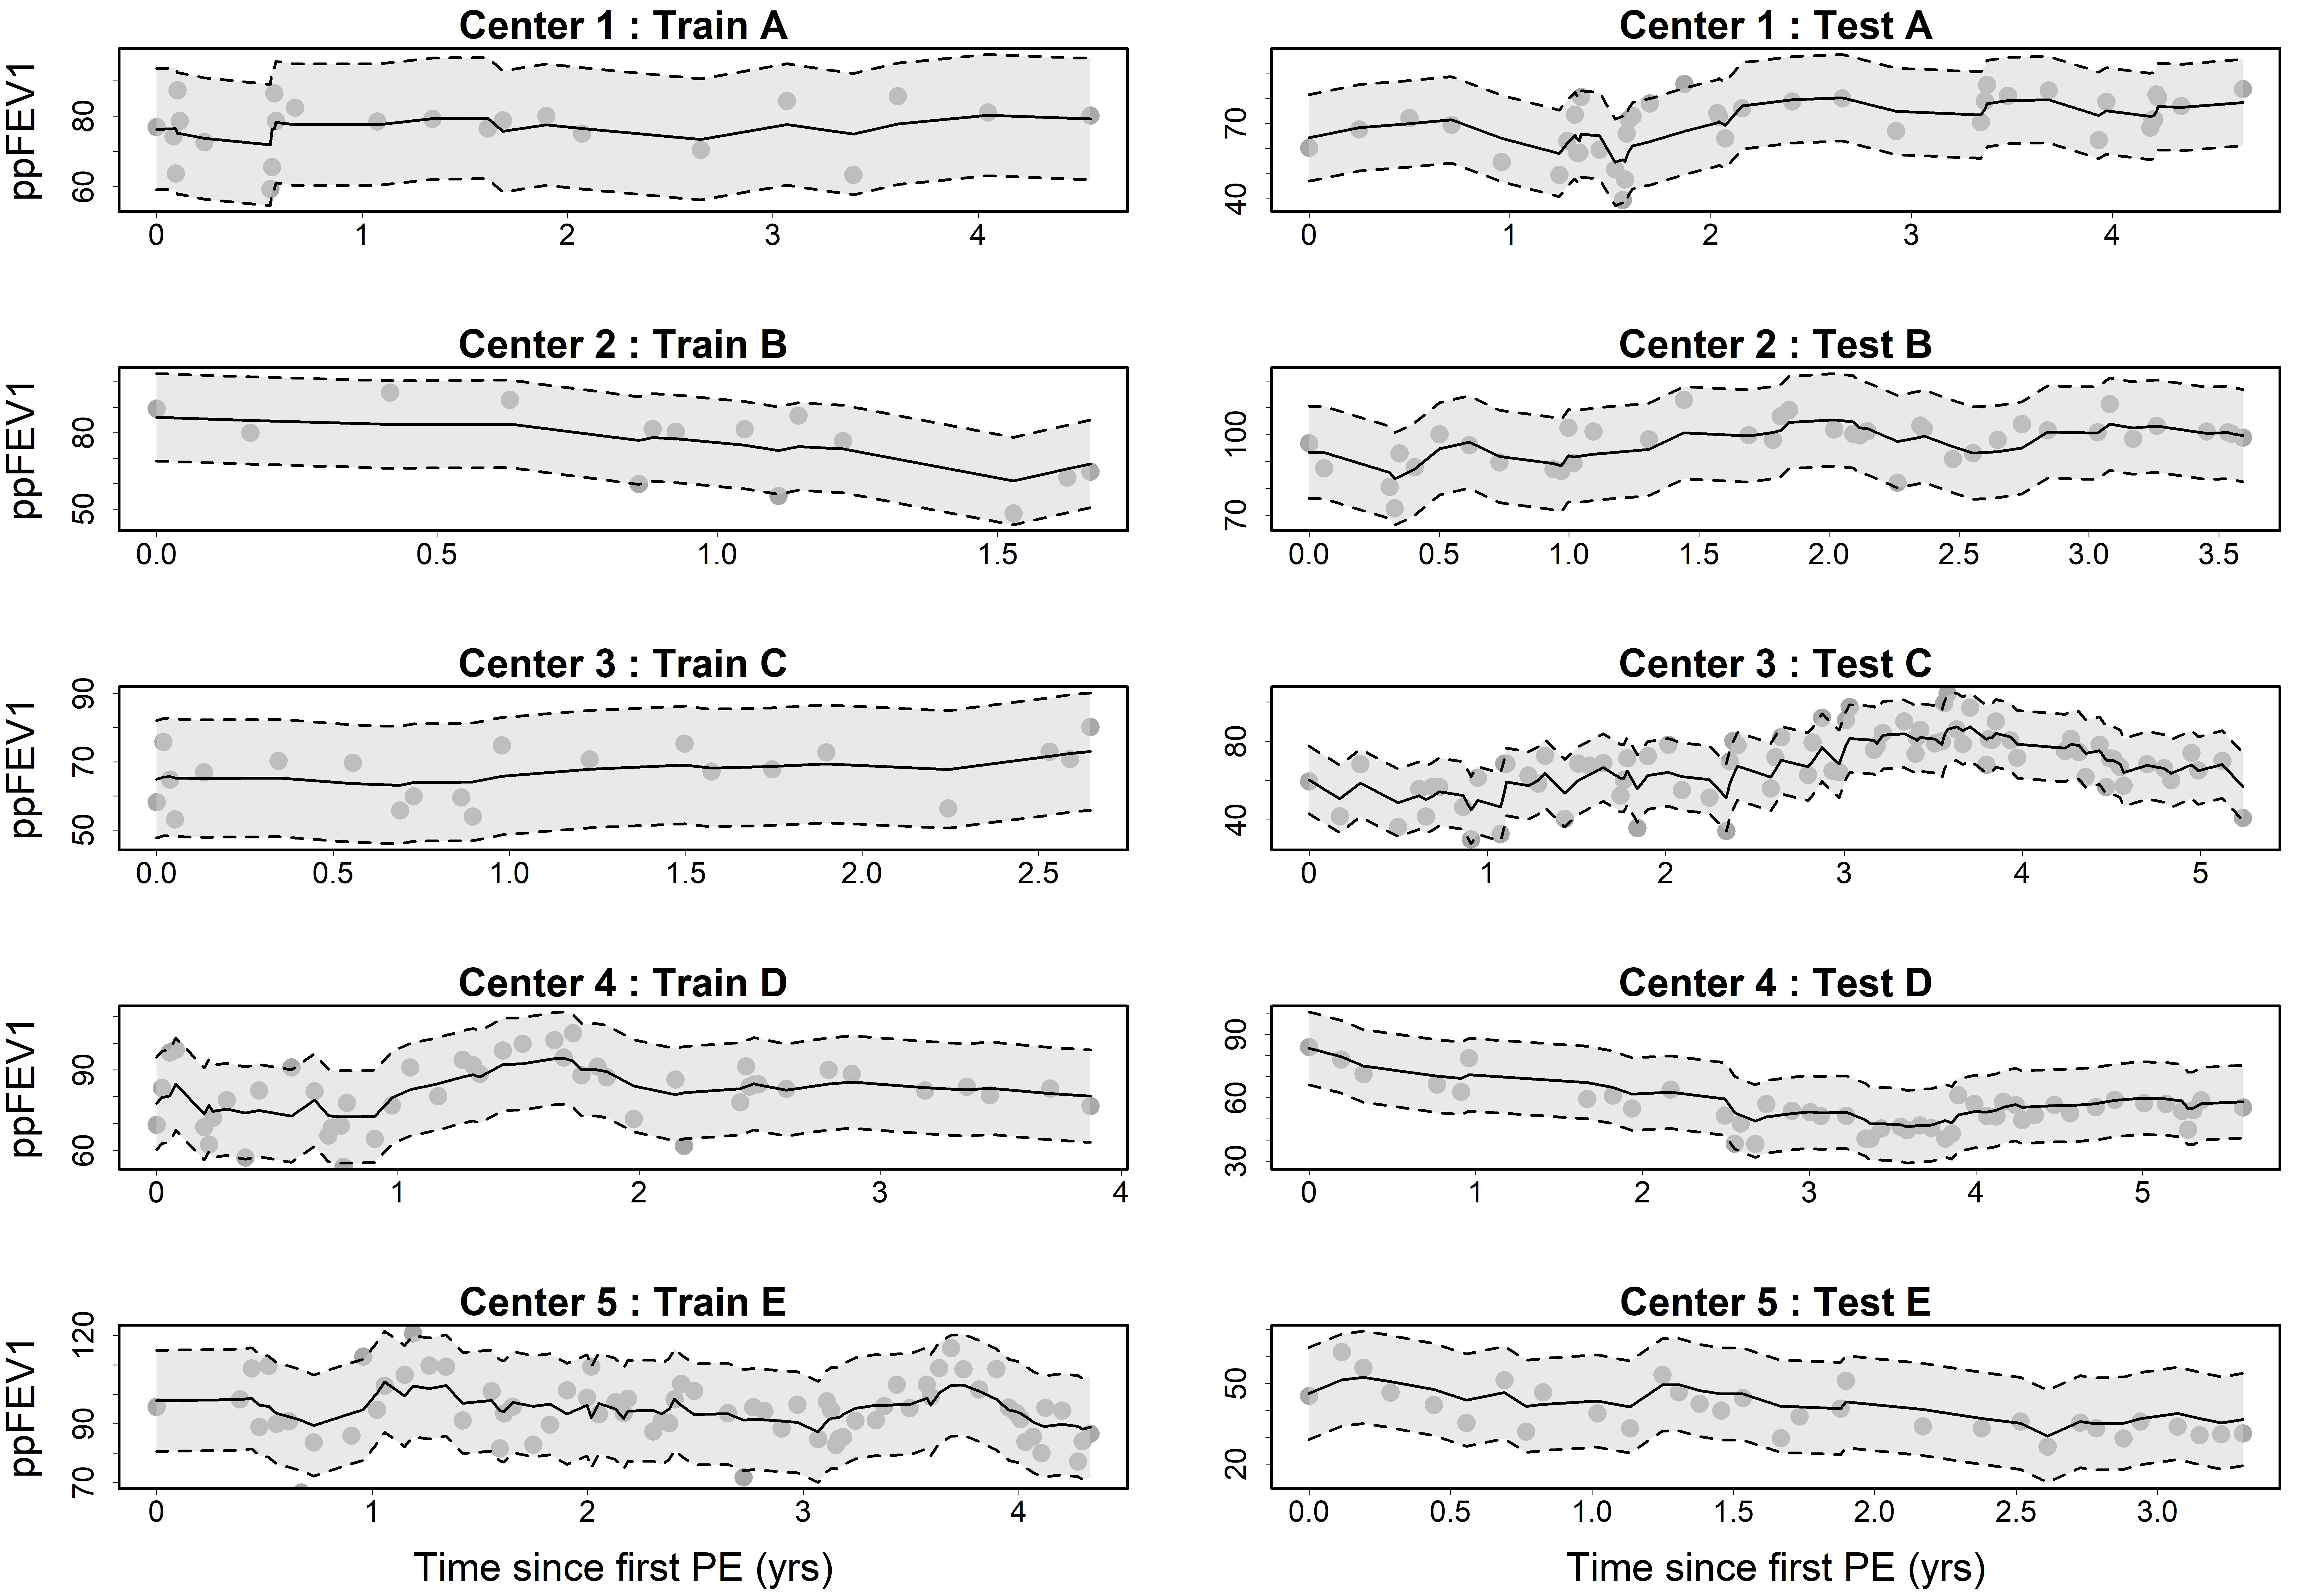
\includegraphics[width=\textwidth]{Figures/Chp2_pred.jpg}
\caption{Prediction for random selected patients from each center under spep-$\mbox{JM}_4$ model, including observed ppFEV1 (gray dots) against time with fitted values (solid lines) and corresponding 95\% CIs (bands)}
\label{fig:pred}
\end{figure}

\begin{figure}[ht]
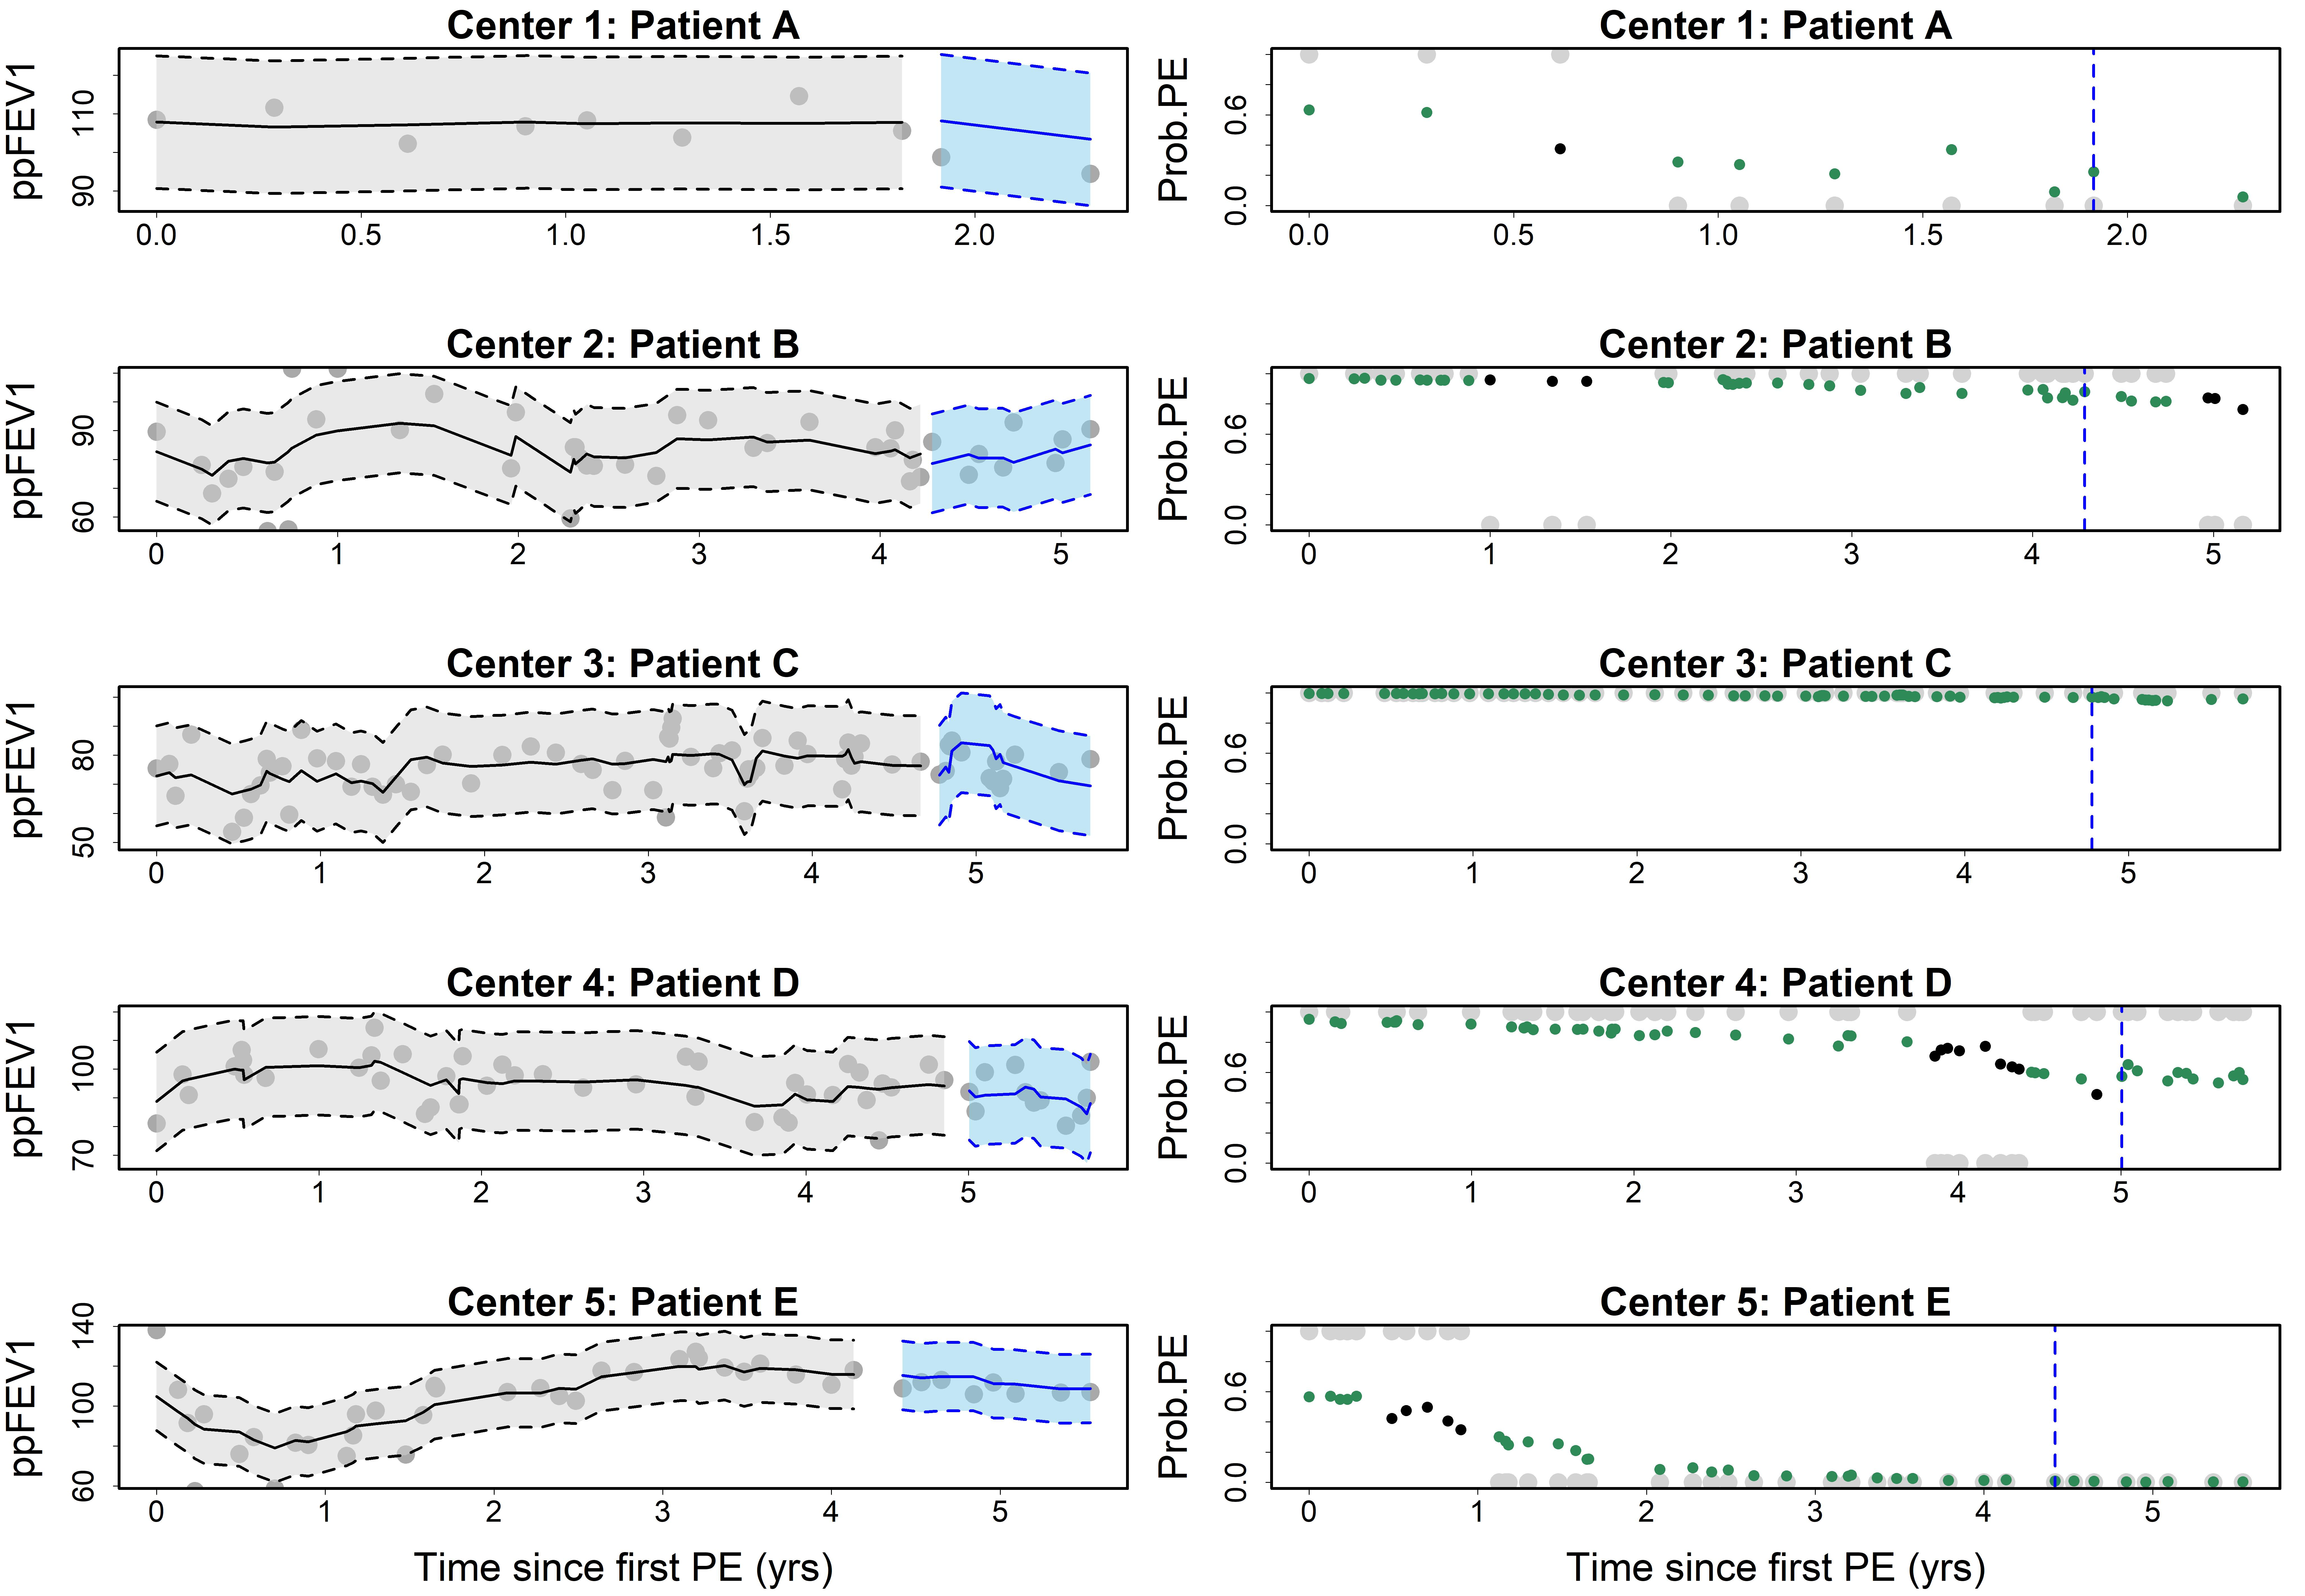
\includegraphics[width=\textwidth]{Figures/Chp2_mask.jpg}
\caption{Forecast for random selected patients from each center under spep-$\mbox{JM}_4$ model, including observed ppFEV1 (gray dots) against time with fitted (solid black lines) and prognostic values (solid blue lines) and corresponding 95\% CIs (bands); observed PE (gray dots) against time with predicted probability of PE onset (green dots for the true classification; black dots for the false classification)}
\label{fig:fcast}
\end{figure}

Table \ref{tab:chp2_pd} shows that spep-$\mbox{JM}_4$ achieves the smallest RMSE and the highest AUC for the training cohort. We note that the difference in accuracy is not evident from spep-$\mbox{JM}_1$ to spep-$\mbox{JM}_4$ for the testing cohort, however, the smallest RMSE is convincing enough to conclude spep-$\mbox{JM}_4$ as the optimal choice. We apply the same training cohort to examine the forecasting performance of each model. Table \ref{tab:chp2_fc} also demonstrates that spep-$\mbox{JM}_4$ is outstanding in forecasting performance. Figure \ref{fig:pred} and \ref{fig:fcast} present individual prediction and forecast under spep-$\mbox{JM}_4$ structure, respectively. Our proposed model is well shown to capture the heterogeneous nature of ppFEV1, whilst provided reasonable predictive probabilities of PE encounters.

\section{Discussion} \label{sec:chp2_con}

In this chapter, we have developed a multilevel Bayesian joint model with a flexible link function to accommodate analysis of longitudinal and binary outcomes for a monitoring CF registry data, which is depicted by hierarchical structures and irregularly observed time points. Our novel approach relaxes the inference on regular clinical follow-up from a previous study \cite{Su2020}, \cite{Su2021}, which avoids unnecessary biases caused by annualized covariates. The rationale for dynamic individual prediction is obtained by plugging posterior means from HMC method into BLUP equations as shown in Section \ref{sec:chp2_pred}. The interplay of Bayesian and frequentist approach is beneficial to both numerical and analytic analysis, especially in modern hierarchical models (\cite{Bayarri2004}). Both the simulation study and motivating example demonstrate the reliable capability of our proposed joint model. Furthermore, our model can be applied to numerous alternative hierarchical data structures, see Section 2 from Brilleman et al. \cite{Brilleman2019} for more data examples. 

For the class of flexible symmetric power link functions, our assessments favor spep over splogit from the model information criterion. In addition, the virtual distinguishes between such two links are presented in Figure \ref{fig:Chp2_cdf_sp}. The authors of the seminal flexible link function (\cite{Jiang2013}) demonstrated that, Equation \ref{eq:ch2_Fsp} achieved left skewness when $0<r<1$; symmetric when $r=1$; right skewness when $r>1$. Researchers need to be aware that this statement cannot hold when values of covariate $x$ are asymmetric (see the simulation study in Appendix \ref{app:b} for details). As a conclusion, we recommend a flexible link function regardless of whether there exists observed skewness of responses in the real data case. 

There may be some possible limitations in this study. We have focused our study on symmetric power link family only, however, an alternative is subject to a class of link functions based on the GEV distribution (\cite{Wang2010}). To the best of our knowledge, there are no existing R packages that incorporate any aforementioned flexible link families, which might be an interesting field to explore in the future research. In addition, given the fact that PE onset would be dependent on various intrinsic factors and CF is a multi-system disease, the aforementioned time-independent association structure can be further extended. Moreover, a joint model of longitudinal and time-to-recurrent outcomes is actively under the investigation with the aim to facilitate the detection of PE.

